% !TEX TS-program = xelatex
% !TEX encoding = UTF-8 Unicode
\documentclass[aspectratio=169,11pt]{beamer}

\usetheme{Madrid}
\usecolortheme{default}
\setbeamertemplate{navigation symbols}{}
\setbeamertemplate{caption}[numbered]

\AtBeginSection[]{
  \begin{frame}[plain,noframenumbering]
    \vfill
    \centering
    {\usebeamercolor[fg]{structure}\bfseries\LARGE\insertsectionhead\par}
    \vfill
  \end{frame}
}

\usepackage{iftex}
\ifPDFTeX
  \usepackage[utf8]{inputenc}
  \usepackage[T1]{fontenc}
  \usepackage{lmodern}
\else
  \usepackage{fontspec}
  \setmainfont{Latin Modern Roman}
  \setsansfont{Latin Modern Sans}
  \setmonofont{Latin Modern Mono}
\fi

\usepackage{microtype}
\usepackage{graphicx}
\usepackage{booktabs}
\usepackage{array}
\usepackage{amsmath}
\usepackage{amssymb}
\usepackage{tikz}
\usetikzlibrary{arrows.meta,positioning}
\usepackage{xurl}

\graphicspath{{../figures/}{../assets/}}

\title[SCRFD Final]{Báo cáo cuối kỳ: SCRFD, SPOS-NAS và ASR+JSAR}
\author[Nhóm 23KHMT]{23127333 Trương Quốc Cường \and 23127011 Lê Anh Duy \and 23127199 Trần Gia Huy}
\institute[HCMUS]{CSC14006 -- Nhận dạng\\Trường ĐH Khoa học Tự nhiên, ĐHQG-HCM}
\date[20/04/2026]{TP. Hồ Chí Minh, ngày 20 tháng 4 năm 2026}
\titlegraphic{
\includegraphics[width=0.15\textwidth]{../assets/HCMUS.png}}

\begin{document}

\begin{frame}
  \titlepage
\end{frame}

\begin{frame}{Mục lục}
  \tableofcontents
\end{frame}

\section{Mở đầu}

\begin{frame}{Phạm vi của báo cáo này}
  \begin{itemize}
    \item Báo cáo chỉ tập trung vào bài báo \textbf{SCRFD} và pipeline detector một giai đoạn cho face detection trên \textbf{WIDER FACE}.
    \item Nội dung được tổ chức theo đúng logic của một report bài báo khoa học: trình bày phương pháp, tái hiện bằng official code, đối chiếu paper với code, rồi phân tích kết quả.
    \item Từ đó nhóm mở rộng theo đúng hai mắt xích quan trọng của SCRFD:
  \end{itemize}
  \begin{block}{Hai hướng mở rộng}
    \textbf{SPOS-NAS} cho bước \textbf{Computation Redistribution};\\[0.15cm]
    \textbf{ASR+JSAR} cho \textbf{việc điều chỉnh tỉ lệ cắt và gán mẫu} trong lúc huấn luyện.
  \end{block}
\end{frame}

\begin{frame}{SCRFD nên được nhìn như pipeline 3 bước}
  \centering
  \resizebox{0.94\textwidth}{!}{%
  \begin{tikzpicture}[
    node distance=0.5cm,
    box/.style={draw, rounded corners, text width=0.29\textwidth, minimum height=1.9cm, align=center, fill=blue!4, font=\footnotesize},
    arrow/.style={-{Latex[length=3mm]}, thick}
  ]
    \node[box] (cr) {\textbf{Bước 1: Computation Redistribution}\\Tìm cấu hình detector ổn trong cùng vùng FLOPs};
    \node[box, right=of cr] (sr) {\textbf{Bước 2: Sample Redistribution}\\Đổi phân bố scale crop khi huấn luyện};
    \node[box, right=of sr] (train) {\textbf{Bước 3: Train / Evaluate}\\Train cấu hình đã chọn và đo AP};
    \draw[arrow] (cr) -- (sr);
    \draw[arrow] (sr) -- (train);
  \end{tikzpicture}%
  }

  \vspace{0.6cm}
  \begin{itemize}
    \item Điểm quan trọng là ba bước này gắn chặt với nhau: kiến trúc đúng nhưng phân phối tỉ lệ cắt khi tăng cường dữ liệu sai vẫn tụt Hard AP.
    \item Vì vậy phần mở rộng cũng phải đi theo đúng trình tự \textbf{CR trước, SR sau}.
  \end{itemize}
\end{frame}

\section{SCRFD Gốc}

\begin{frame}{Bài toán mà SCRFD giải}
  \begin{itemize}
    \item SCRFD hướng vào \textbf{face detection hiệu quả}, đặc biệt là nhóm \textbf{tiny faces} trong ảnh VGA.
    \item Trên WIDER FACE, split Hard chứa rất nhiều mặt cực nhỏ, nên detector không thể chỉ mạnh về ngữ nghĩa sâu; nó còn phải giữ tốt chi tiết không gian ở các tầng nông.
    \item Bài báo vì thế không chỉ hỏi mô hình nào mạnh hơn, mà hỏi hai câu đúng hơn:
  \end{itemize}
  \begin{block}{Hai câu hỏi cốt lõi}
    Với cùng ngân sách FLOPs, compute nên đặt ở đâu?\\
    Và trong lúc train, detector nên nhìn thấy khuôn mặt ở những scale nào nhiều hơn?
  \end{block}
\end{frame}

\begin{frame}{Minh họa WIDER FACE Hard và tiny faces}
  \begin{figure}
    \centering
    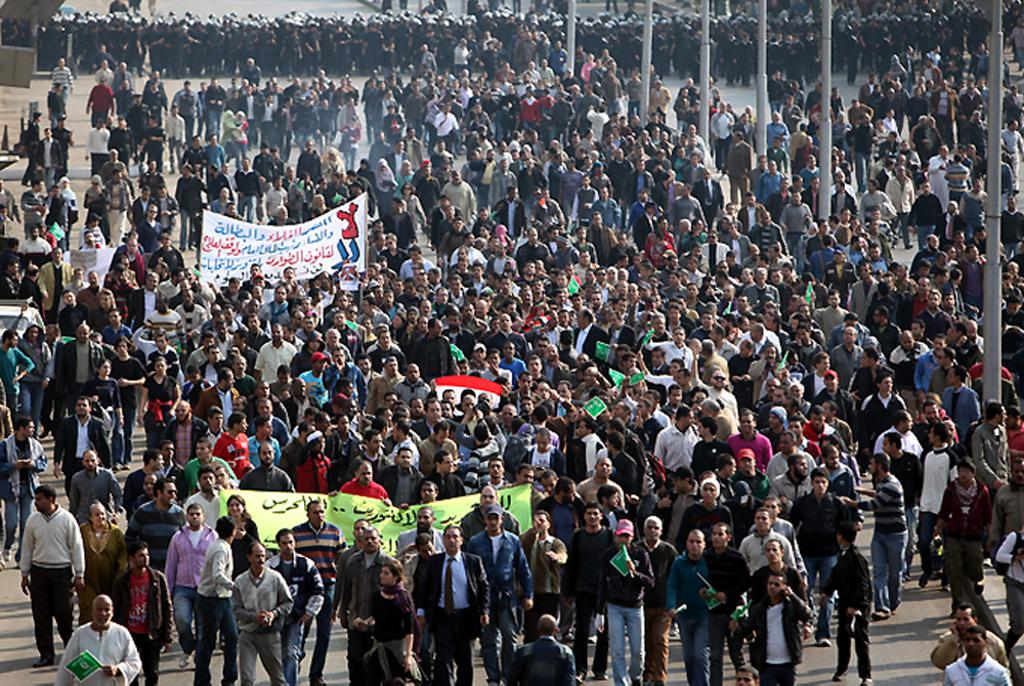
\includegraphics[width=0.98\linewidth,height=0.82\textheight,keepaspectratio]{widerface_hard_example.jpg}
  \end{figure}
\end{frame}

\begin{frame}{Kiến trúc nền Backbone--Neck--Head}
  \begin{itemize}
    \item \textbf{Backbone}: tạo chuỗi đặc trưng \(C_2 \rightarrow C_5\).
    \item \textbf{PAFPN}: hợp nhất thông tin nhiều mức để vừa giữ vị trí vừa giữ ngữ nghĩa.
    \item \textbf{Dense head}: dự đoán classification và bbox trên các feature map.
    \item Trọng tâm của SCRFD là làm cho cấu trúc này phù hợp hơn với tiny-face detection thay vì bê nguyên detector phân loại ảnh sang.
  \end{itemize}
\end{frame}

\begin{frame}{Minh họa kiến trúc Backbone--Neck--Head}
  \begin{figure}
    \centering
    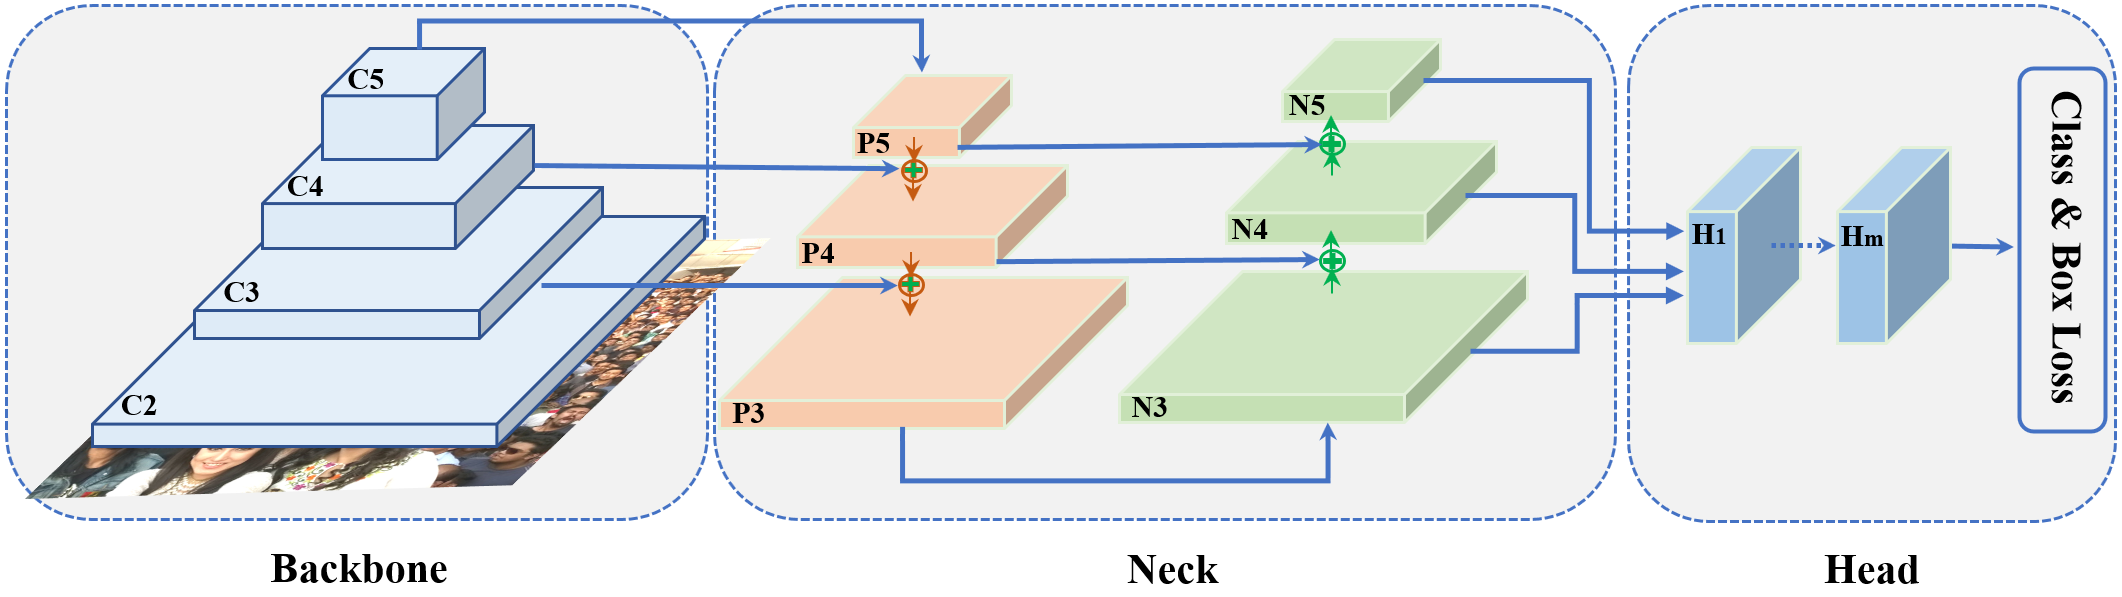
\includegraphics[width=0.98\linewidth,height=0.82\textheight,keepaspectratio]{scrfd_backbone_neck_head.png}
  \end{figure}
\end{frame}

\begin{frame}{Computation Redistribution được làm theo hai pha}
  \begin{itemize}
    \item \textbf{Pha 1: search backbone.} Mục tiêu là cô lập câu hỏi riêng cho backbone: trong khung 4 stage \(C_2,C_3,C_4,C_5\), compute nên dồn nhiều hơn vào stage nào.
    \item Ở repo public demo, bước này mặc định sinh \textbf{64 candidate backbone}; paper mô tả quy mô đầy đủ là \textbf{320 candidate}.
    \item Mỗi candidate đều bị lọc lại theo cùng vùng chi phí, trong code là khoảng \textbf{target FLOPs \(\pm\) 2\%}, nên chỉ những cấu hình còn quanh 2.5G mới được giữ lại để train và so sánh.
    \item Các cấu hình hợp lệ sau đó được \textbf{train rút gọn 80 epoch}, đánh giá bằng \textbf{Hard mAP}, rồi chọn \textbf{config tốt nhất} làm template cho pha 2.
    \item \textbf{Không có bước lấy top 10\% hay khoảng tin cậy thống kê}; đây là ranking-based search: sinh candidate \(\rightarrow\) lọc FLOPs \(\rightarrow\) train ngắn \(\rightarrow\) chọn config thắng.
  \end{itemize}
\end{frame}

\begin{frame}[shrink=8]{Các bậc tự do mà CR thực sự đi tìm}
  \begin{itemize}
    \item \textbf{Pha 1 -- search backbone:} không search từ số 0, mà đi trong một khung 4 stage cố định rồi thay đổi các bậc tự do chính của backbone.
    \item Các bậc tự do ở bước này là: \textbf{loại block}, \textbf{base width ban đầu}, \textbf{độ sâu từng stage}, và \textbf{tỉ lệ độ rộng giữa các stage}.
    \item Nói ngắn gọn, pha 1 đang đi tìm \textbf{hình dạng backbone}: stage nào sâu hơn, stage nào rộng hơn, và độ dốc tăng width giữa \(C_2 \rightarrow C_5\) nên như thế nào.
    \item \textbf{Pha 2 -- search toàn mạng:} từ backbone template thắng ở pha 1, paper không mở toàn bộ detector một cách tự do, mà chỉ cho backbone dao động quanh template đó rồi tinh chỉnh tiếp \textbf{neck} và \textbf{head}.
    \item Các bậc tự do ở bước này là: \textbf{mức scale lại độ sâu backbone}, \textbf{mức scale lại độ rộng backbone}, \textbf{số kênh của neck}, \textbf{số kênh của head}, và \textbf{độ sâu của head}.
    \item Ý nghĩa của cách tách này là tránh để neck/head che mờ tín hiệu thật sự của backbone ở đầu quy trình, rồi chỉ sau đó mới phân bổ nốt compute cho toàn detector.
  \end{itemize}
\end{frame}

\begin{frame}{Quy trình tìm kiếm kiến trúc CR}
  \begin{figure}
    \centering
    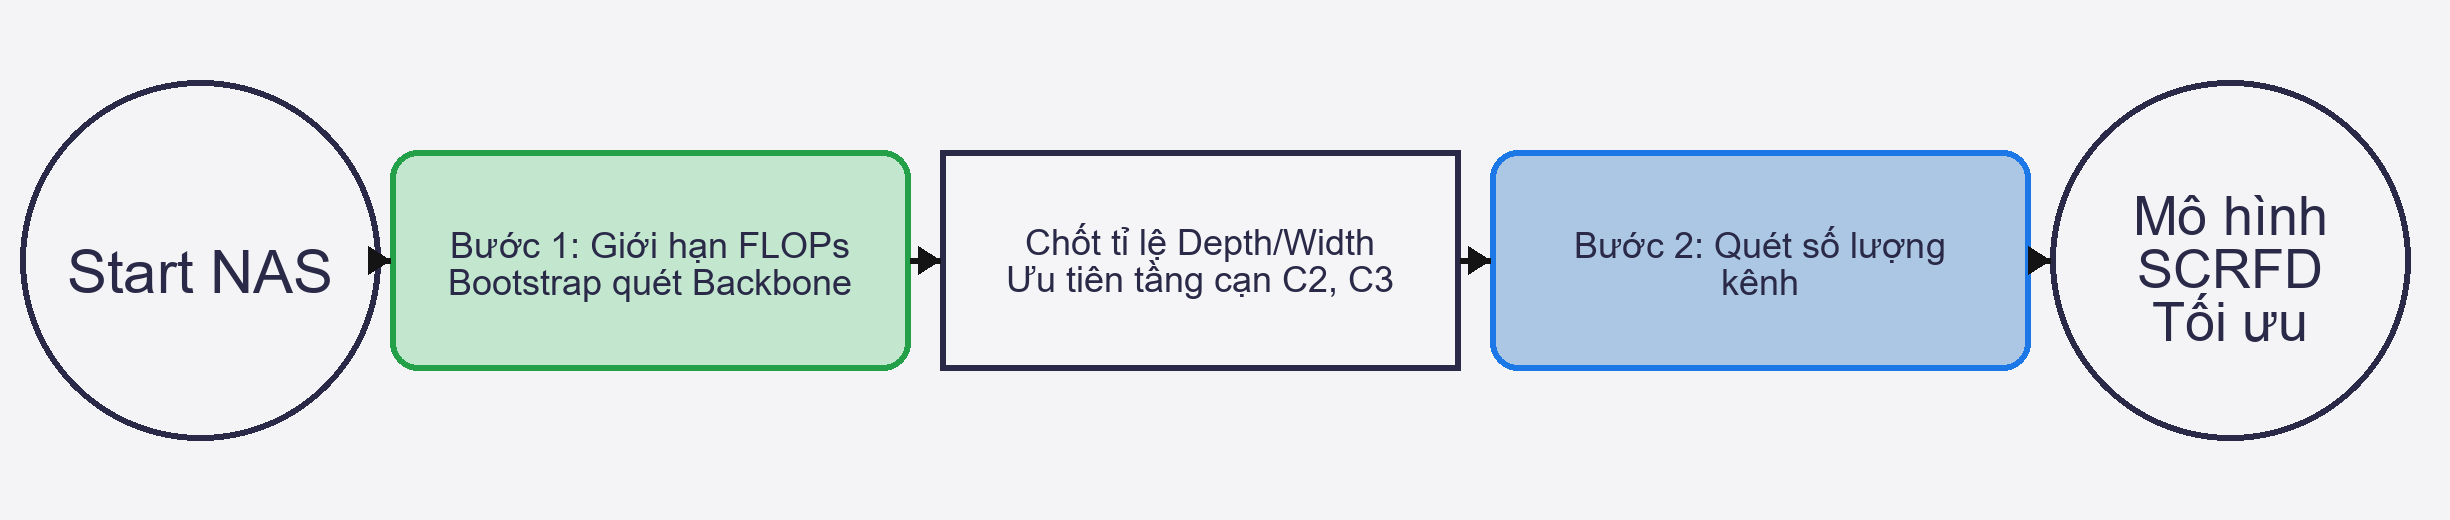
\includegraphics[width=0.98\linewidth,height=0.82\textheight,keepaspectratio]{scrfd_two_step_nas_flow.png}
  \end{figure}
\end{frame}

\begin{frame}{Giả định và giới hạn của CR}
  \begin{itemize}
    \item CR không search từ số 0. Paper giả định trước một \textbf{khung detector cố định}: backbone 4 stage, PAFPN, dense head, các mức stride chính vẫn giữ nguyên.
    \item Trong pha backbone, search thực chất là phân bổ lại depth/width quanh template ban đầu, chứ không mở tự do mọi loại module.
    \item Trong pha toàn mạng, detector cũng không được mở hoàn toàn; backbone đã bị khóa quanh template thắng, rồi mới phân phối nốt compute cho neck và head.
    \item Vì vậy giá trị của CR không phải ở chỗ paper search mọi thứ, mà ở chỗ paper chọn đúng abstraction level để search: \textbf{phân bổ compute giữa các phần của detector}.
  \end{itemize}
\end{frame}

\begin{frame}{Sample Redistribution tác động vào đâu}
  \begin{enumerate}
    \item Mỗi ảnh train được crop vuông theo một scale rồi resize về cùng input \(640 \times 640\).
    \item Vì vậy cùng một khuôn mặt sau resize có thể lớn hơn hoặc nhỏ hơn tương đối, dù ảnh đầu vào là cùng một ảnh.
    \item Kích thước tương đối đó quyết định mặt rơi vào feature level nào và có bao nhiêu positive anchors.
    \item Do đó SR không chỉ là augmentation; nó đang điều khiển trực tiếp \textbf{training signal} cho tiny/small faces.
  \end{enumerate}
  \begin{block}{Luồng nhân quả}
    bộ tỉ lệ cắt \(\rightarrow\) face size sau resize \(\rightarrow\) positive samples \(\rightarrow\) Hard AP
  \end{block}
\end{frame}

\begin{frame}{Giả định và giới hạn của SR}
  \begin{itemize}
    \item SR cũng không tối ưu trực tiếp mật độ mẫu dương; paper chỉ search trên một \textbf{tập tỉ lệ cắt rời rạc} rồi để pipeline crop/resize biến nó thành tín hiệu học.
    \item Nghĩa là paper tối ưu một biến gián tiếp: bộ tỉ lệ cắt, chứ không tối ưu trực tiếp số mẫu dương hay gradient mass theo level.
    \item Public release còn cho thấy narrative của paper và code public không hoàn toàn trùng nhau: code công khai giữ một danh sách tỉ lệ cắt dựng tay, trong khi paper nhấn mạnh bộ tỉ lệ cắt được tìm ra.
    \item Điểm này rất quan trọng khi đọc kết quả reproduction: chênh lệch Hard AP có thể đến từ chính phân phối tỉ lệ cắt khi tăng cường dữ liệu, không chỉ từ backbone hay random seed.
  \end{itemize}
\end{frame}

\begin{frame}{Điểm mạnh và hạn chế của SCRFD}
  \begin{columns}[T,onlytextwidth]
    \column{0.49\textwidth}
    \begin{block}{Điểm mạnh}
      \begin{itemize}
        \item Đặt đúng bài toán tiny-face detection dưới ràng buộc hiệu quả.
        \item Nối được kiến trúc và dữ liệu train thành một pipeline logic.
        \item Đường cong accuracy-efficiency rất thực dụng cho face detection.
      \end{itemize}
    \end{block}
    \column{0.49\textwidth}
    \begin{block}{Hạn chế}
      \begin{itemize}
        \item Search vẫn tốn tài nguyên.
        \item Search space còn bị ràng buộc bởi template detector ban đầu.
        \item Kết quả gắn rất mạnh với WIDER FACE và tiny-face benchmark.
      \end{itemize}
    \end{block}
  \end{columns}
\end{frame}

\section{Reproduction}

\begin{frame}{WIDER FACE là benchmark trung tâm của báo cáo}
  \small
  \begin{tabular}{@{}lccc@{}}
    \toprule
    Split & Số ảnh & Số face boxes & Ghi chú \\
    \midrule
    Train & 12,880 & 159,393 & dùng để train \\
    Val & 3,226 & 39,697 & dùng để evaluate \\
    Test & 16,097 & -- & không có GT public \\
    \bottomrule
  \end{tabular}

  \vspace{0.35cm}
  \begin{itemize}
    \item Paper thực chất bám rất chặt vào WIDER FACE để search, train và benchmark.
    \item EDA trong report cho thấy hơn 70\% face boxes nằm dưới ngưỡng \(32\) px, nên tiny faces không phải edge case mà là vùng dữ liệu thống trị bài toán.
  \end{itemize}
\end{frame}

\begin{frame}{Cấu hình baseline chạy lại paper}
  \begin{itemize}
    \item Nhóm bám \textbf{official public SCRFD codebase} và official detector family, không tự viết lại mô hình.
    \item Baseline được chọn là \textbf{SCRFD-2.5GF}: đủ lớn để có ý nghĩa thống kê, nhưng vẫn nằm trong phạm vi tài nguyên có thể tái hiện ổn định.
    \item Đây là quyết định có chủ ý: full NAS của paper quá nặng vì phải sinh nhiều candidate, train rút gọn, đánh giá, chọn cấu hình rồi mới train dài cho model cuối.
    \item Bộ 12 mức tỉ lệ cắt theo bài báo được nhóm \textbf{phục dựng lại} trên pipeline công khai; nó không phải một baseline upstream có sẵn đúng nguyên xi từ authors.
    \item Vì vậy reproduction của nhóm là \textbf{public reproducible baseline trên official stack}, không phải rerun toàn bộ NAS end-to-end của paper.
  \end{itemize}
\end{frame}

\begin{frame}{Protocol train và evaluate của baseline}
  \small
  \begin{tabular}{@{}p{0.30\textwidth}p{0.62\textwidth}@{}}
    \toprule
    Thành phần & Thiết lập \\
    \midrule
    Input & \(640 \times 640\) \\
    Optimizer & SGD, momentum \(0.9\), weight decay \(5\times10^{-4}\) \\
    Schedule & 80 epochs, cosine LR, warmup \\
    Augmentation & crop vuông, resize, flip, photometric distortion, normalize \\
    Evaluation & WIDER FACE Easy/Medium/Hard trên \textbf{validation split}, threshold \(0.02\), NMS \(0.45\) \\
    \bottomrule
  \end{tabular}

  \vspace{0.3cm}
  \begin{itemize}
    \item Điểm cần nhớ là baseline dùng cùng pipeline train/eval với official repo, nhưng đường chạy `80e cosine + bộ 12 mức theo bài báo` là cấu hình thực nghiệm nhóm dựng lại trên official stack.
    \item Vì vậy khi so với official model zoo, phải tách rõ hai lớp nguyên nhân: khác recipe train dài-ngắn và khác phân phối tỉ lệ cắt khi tăng cường dữ liệu.
  \end{itemize}
\end{frame}

\begin{frame}{Kết quả tái hiện baseline và vai trò của bộ 12 mức theo bài báo}
  \small
  \begin{tabular}{@{}lcccc@{}}
    \toprule
    Thiết lập & Easy & Medium & Hard & mAP \\
    \midrule
    Official model zoo & 93.78 & 92.16 & 77.87 & 87.94 \\
    Baseline (bộ mặc định) & 91.40 & 89.69 & 72.49 & 84.53 \\
    Baseline (12 mức theo bài báo) & 91.61 & 89.99 & 73.71 & 85.10 \\
    \bottomrule
  \end{tabular}

  \vspace{0.35cm}
  \begin{itemize}
    \item Trong cùng khung \textbf{80 epoch cosine}, chỉ riêng việc đổi sang \textbf{bộ 12 mức theo bài báo} đã kéo Hard AP tăng \(+1.22\).
    \item Điều này xác nhận một insight lớn của report: phần khó nhất của SCRFD không chỉ là chạy model, mà là tái tạo đúng phân phối tỉ lệ cắt cho tiny faces.
  \end{itemize}
\end{frame}

\begin{frame}{Đọc đúng gap với official model zoo}
  \begin{itemize}
    \item Gap với official không nên quy hết cho một lý do duy nhất.
    \item \textbf{Official 2.5GF} là mốc model zoo đã được huấn luyện rất dài trong public recipe gốc, khoảng \textbf{640 epoch với step schedule}.
    \item \textbf{Baseline của nhóm} là \textbf{80 epoch với cosine scheduler} trên official public codebase, rồi gắn thêm bộ 12 mức theo bài báo vào pipeline công khai.
    \item Vì vậy gap Hard \(-4.16\) phải được đọc như tổng hợp của:
  \end{itemize}
  \begin{block}{Bốn nguồn chênh lệch}
    training horizon, scale policy, randomness, và mức độ tinh chỉnh sâu hơn của pipeline official
  \end{block}
\end{frame}

\section{SPOS-NAS Cho CR}

\begin{frame}{Vì sao dùng SPOS-NAS để mở rộng CR}
  \begin{itemize}
    \item Official CR search rất nặng, nên nhóm dùng \textbf{SPOS-NAS proxy} để khảo sát sâu hơn cấu trúc phân bổ compute trong cùng miền 2.5 GFLOPs.
    \item Mục tiêu không phải thay official AP benchmark, mà là kiểm tra xem khi search dưới áp lực tiny-face detection, winner có tự học một quy luật phân bổ compute nhất quán hay không.
    \item Đây là \textbf{phân tích bổ sung cho CR}, không phải nhánh evidence chính mạnh hơn baseline + ASR.
    \item Đây là phần mở rộng trực tiếp cho \textbf{Computation Redistribution}, nên được trình bày trước.
  \end{itemize}
\end{frame}

\begin{frame}{Flow triển khai SPOS-NAS proxy}
  \begin{enumerate}
    \item Xây dựng một supernet bao phủ nhiều phương án depth/width trên bốn stage \(C_2 \rightarrow C_5\).
    \item Huấn luyện supernet theo kiểu single-path để mỗi mini-batch chỉ kích hoạt một đường con.
    \item Sau khi supernet đủ ổn định, lấy mẫu \textbf{1,000} candidate trong cùng vùng 2.5 GFLOPs.
    \item Với mỗi candidate, chạy BatchNorm recalibration rồi đo proxy score trên validation.
    \item Phân tích cấu hình Top-10 / thua để rút ra quy luật.
  \end{enumerate}
\end{frame}

\begin{frame}{Minh họa luồng làm việc của SPOS}
  \begin{figure}
    \centering
    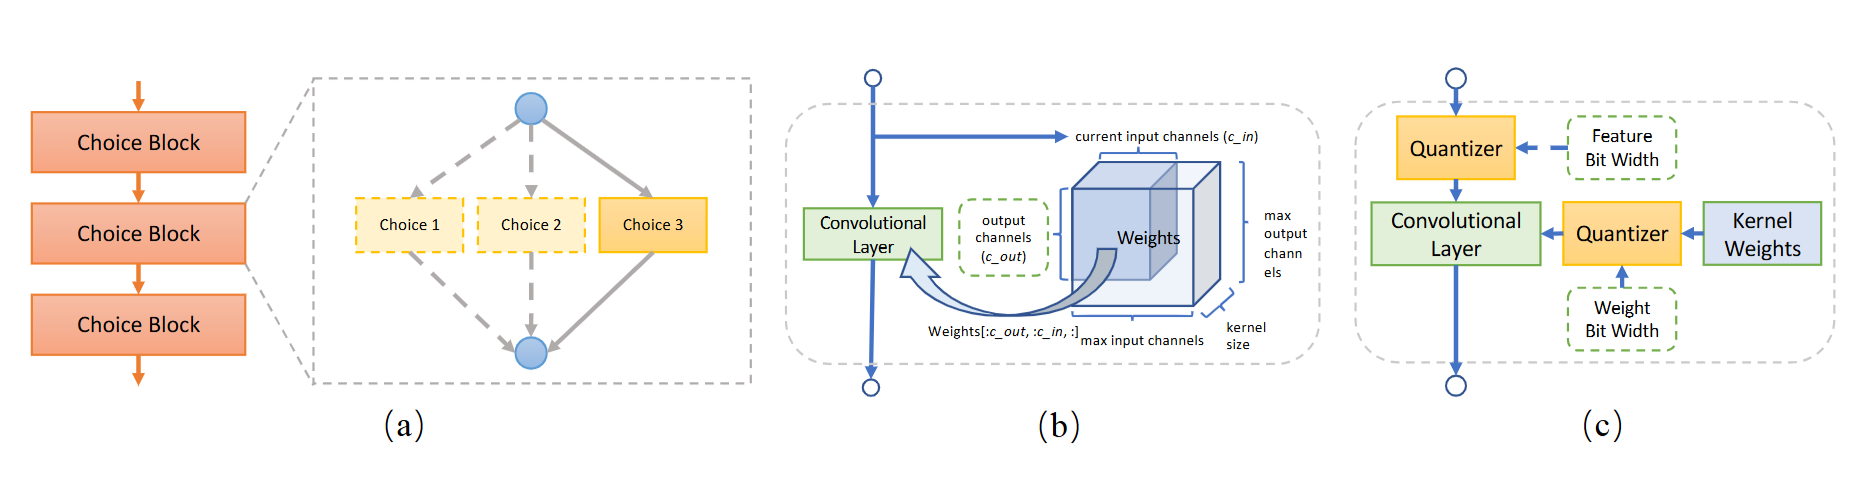
\includegraphics[width=0.98\linewidth,height=0.82\textheight,keepaspectratio]{SPOS-Workflow-viz.png}
  \end{figure}
\end{frame}

\begin{frame}{Inference heatmap của kiến trúc tốt nhất}
  \begin{figure}
    \centering
    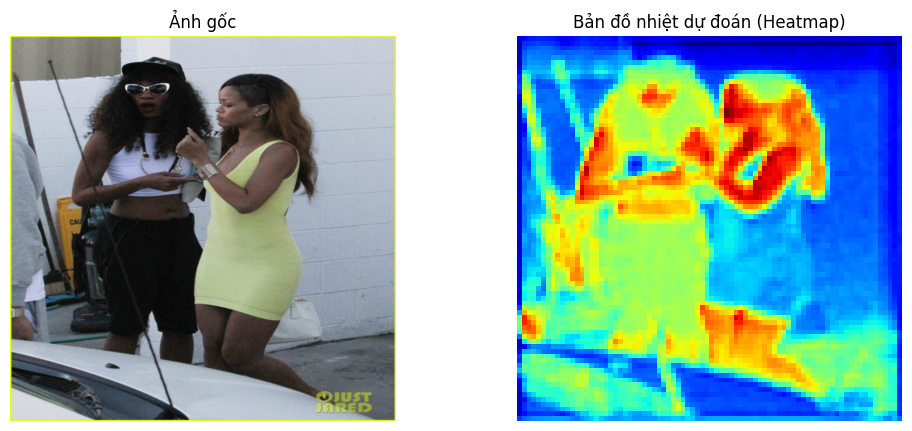
\includegraphics[width=0.98\linewidth,height=0.82\textheight,keepaspectratio]{spos_best_architecture_heatmap.png}
  \end{figure}
\end{frame}

\begin{frame}{Ví dụ heatmap generated theo edge-focus}
  \begin{figure}
    \centering
    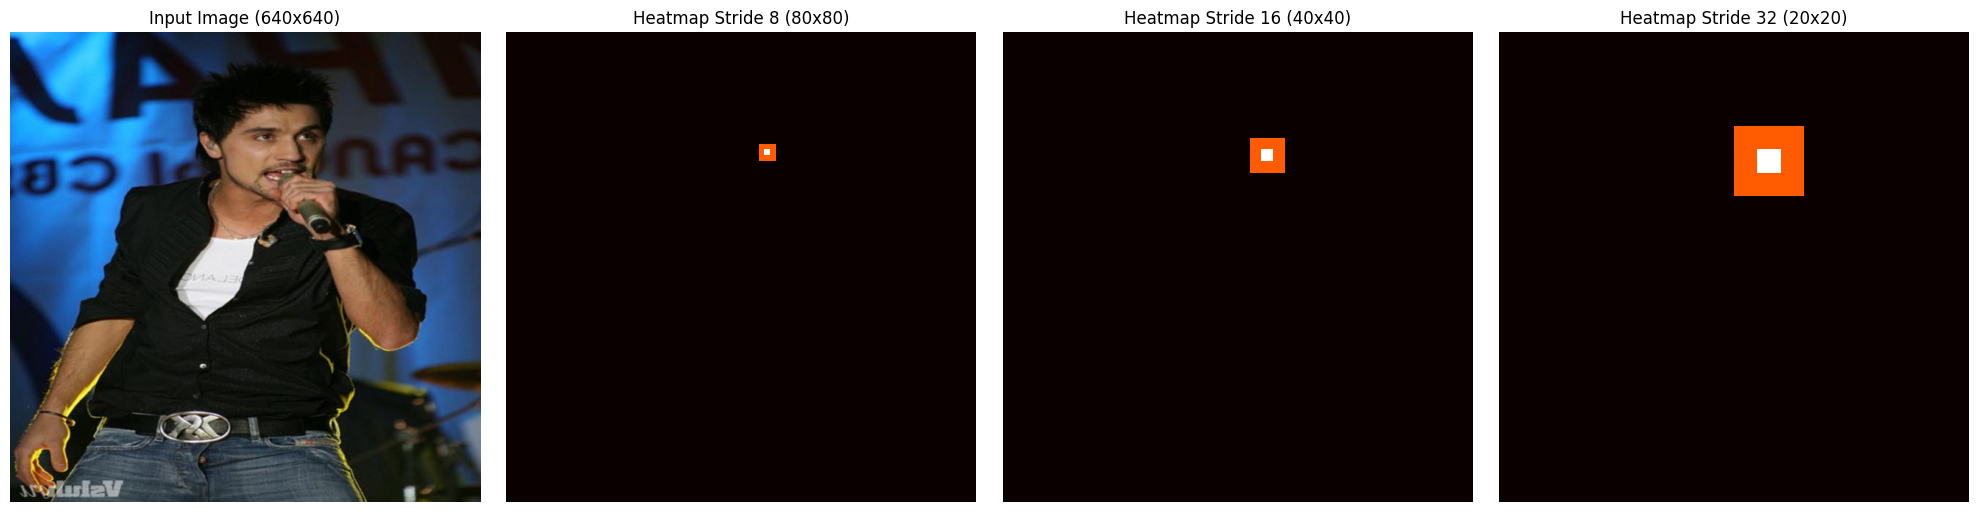
\includegraphics[width=0.98\linewidth,height=0.82\textheight,keepaspectratio]{spos_center_focus_heatmap_example.png}
  \end{figure}
\end{frame}

\begin{frame}{Ví dụ heatmap ngược lại theo center-focus}
  \begin{figure}
    \centering
    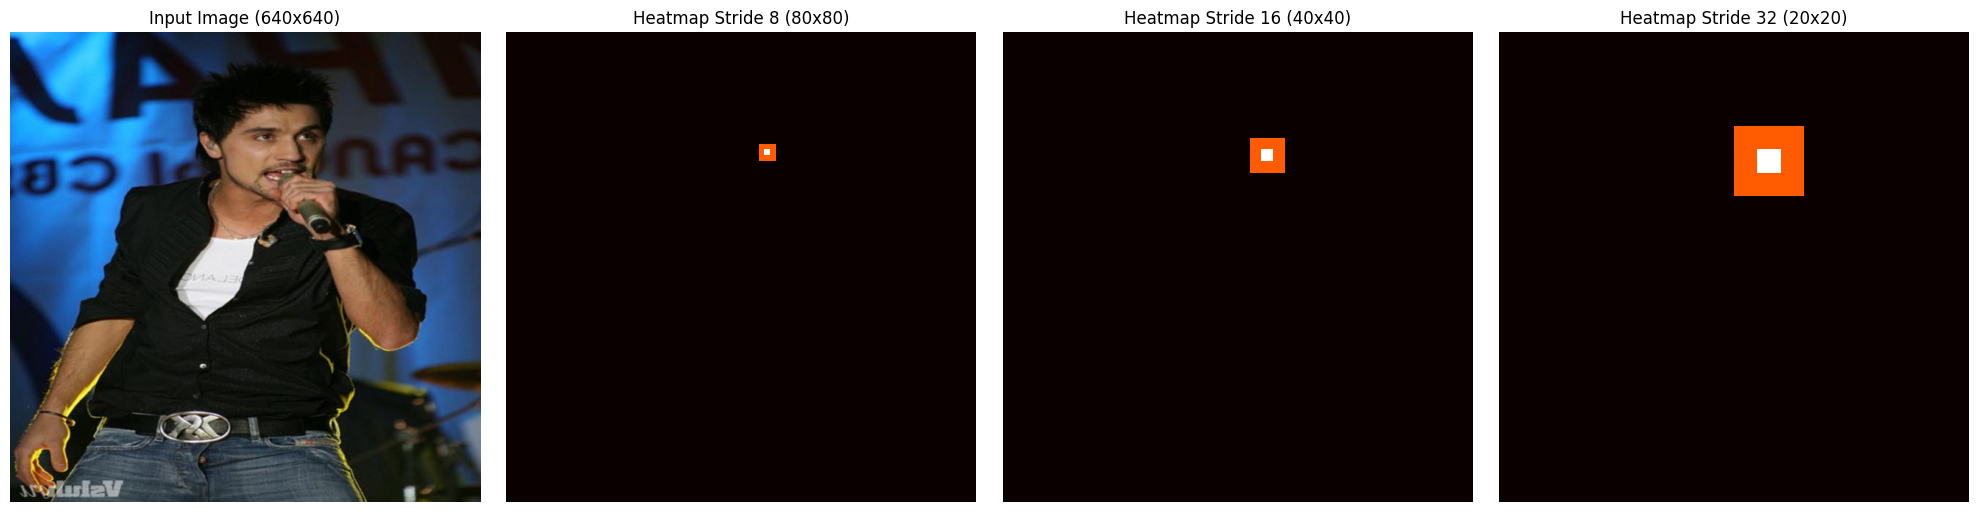
\includegraphics[width=0.98\linewidth,height=0.82\textheight,keepaspectratio]{spos_center_focus_heatmap_example.png}
  \end{figure}
\end{frame}

\begin{frame}{Đánh giá Supernet và Proxy NAS}
  \begin{itemize}
    \item Cả supernet center-focus và edge-focus đều hội tụ ổn định sau khi giảm LR.
    \item Quá trình lấy mẫu sinh ra không gian biến thể bao phủ rất đều đặn, rải rác công bằng cơ hội thay đổi cấu trúc cho mọi tầng.
    \item Bảng xếp hạng 1,000 candidates cho thấy sự phân hóa rõ rệt dù cùng GFLOPs, tạo cơ sở mạnh để chọn lọc cấu hình tối ưu.
  \end{itemize}
\end{frame}

\begin{frame}{Tính đồng đều của không gian Search (Uniformity)}
  \begin{figure}
    \centering
    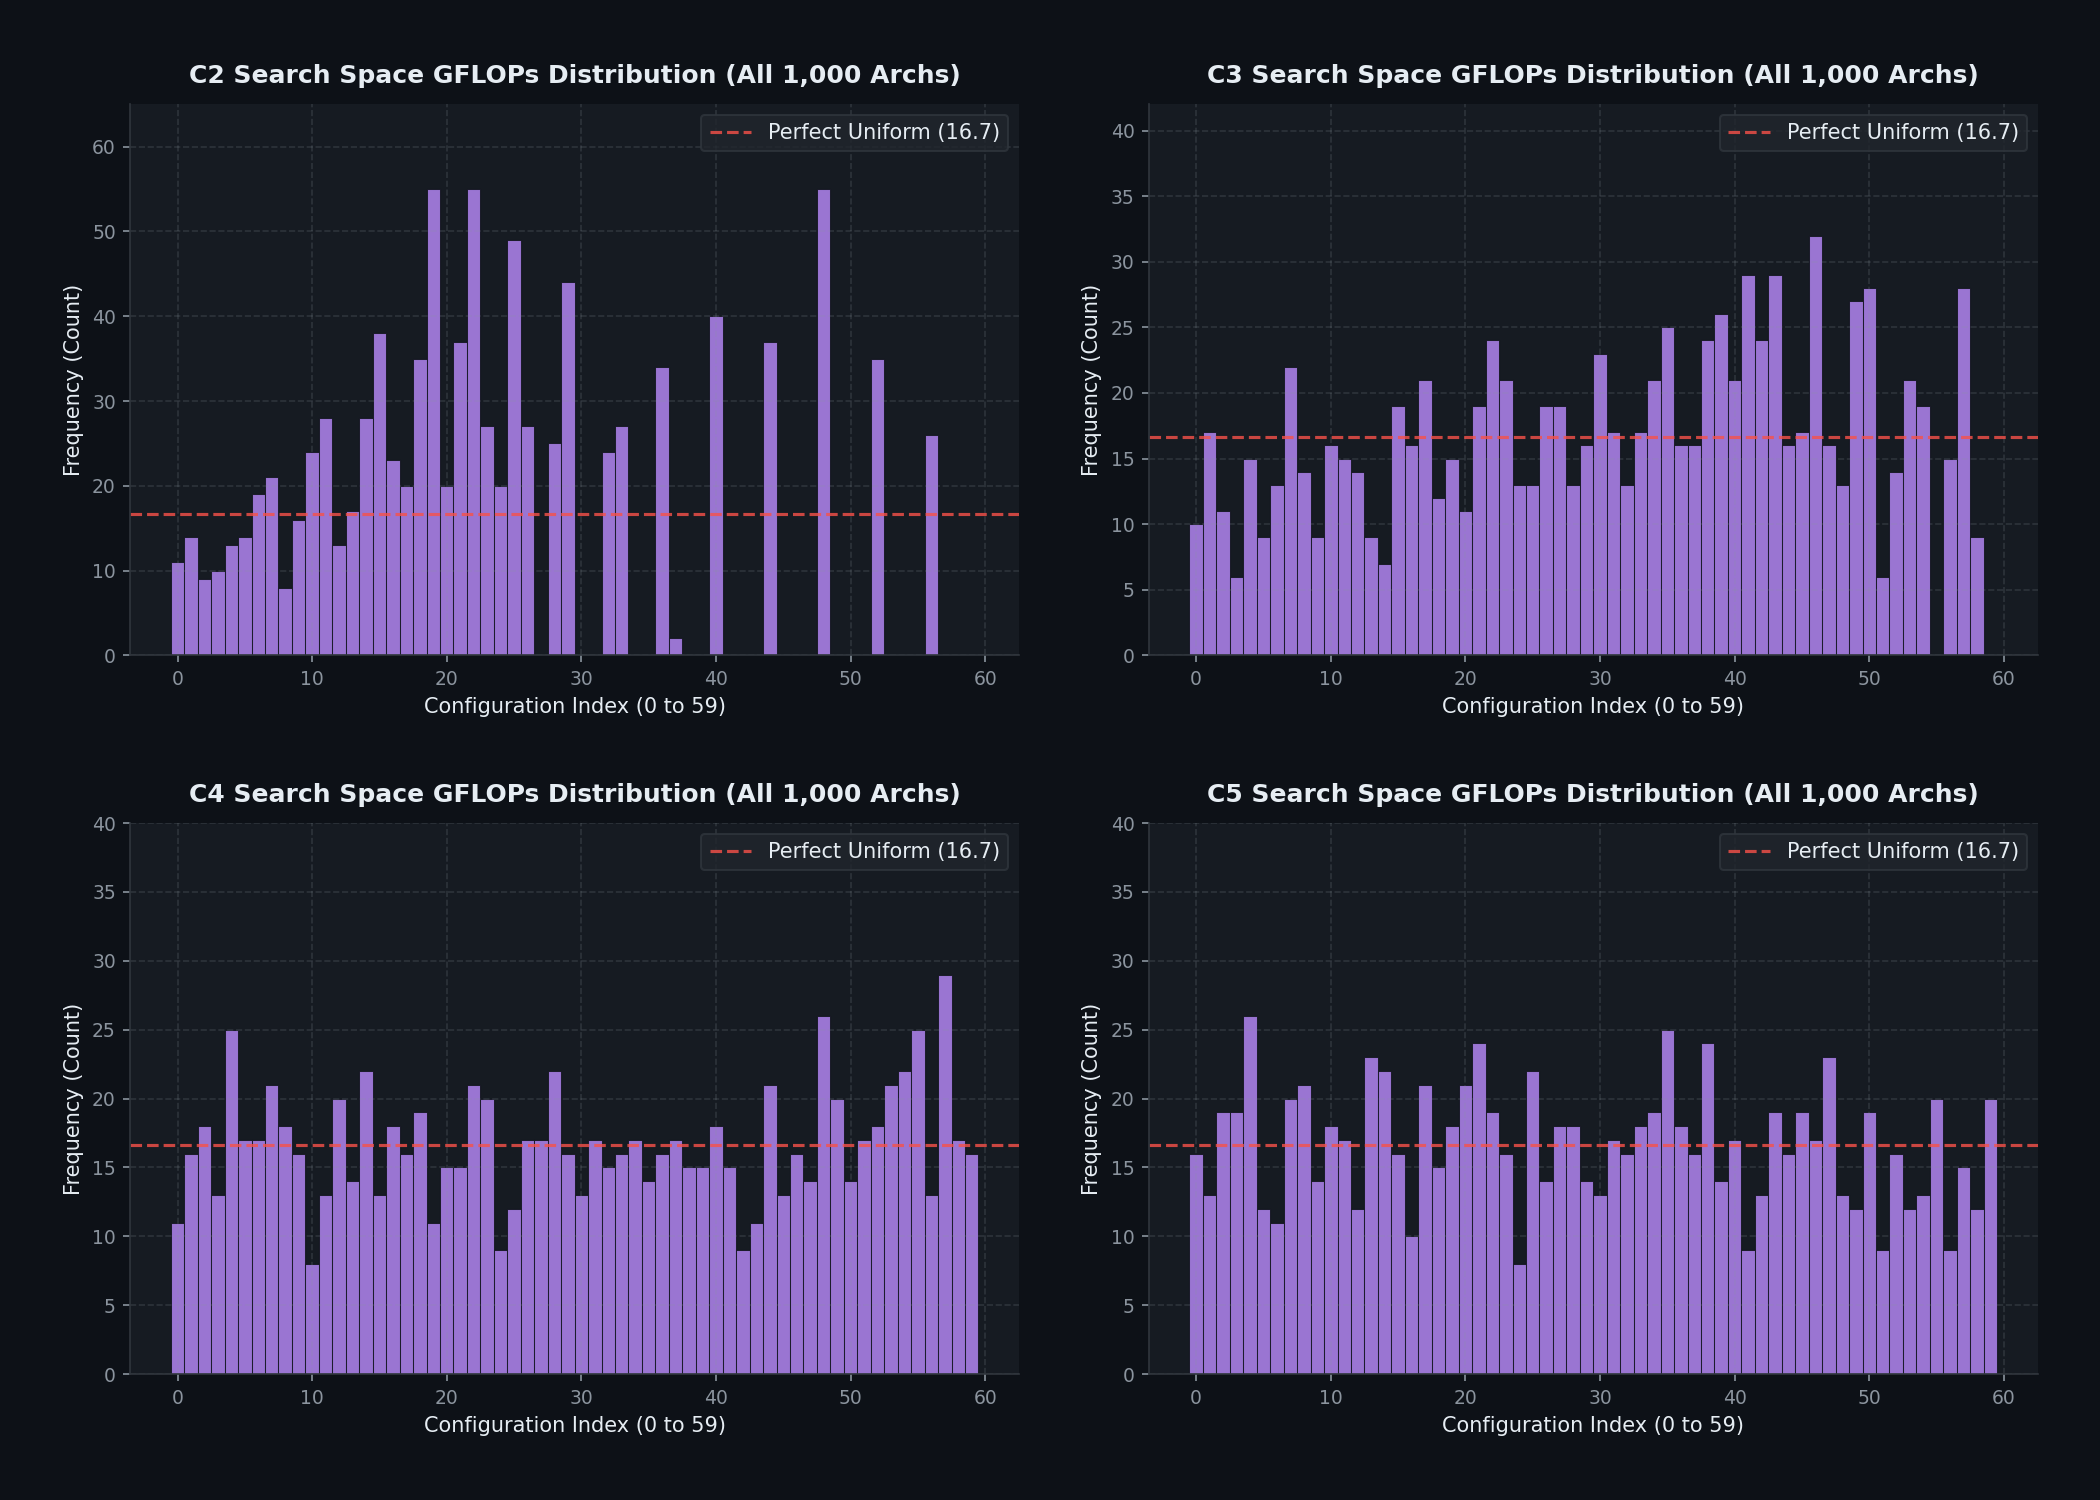
\includegraphics[width=0.98\linewidth,height=0.82\textheight,keepaspectratio]{fig_search_space_uniformity.png}
  \end{figure}
\end{frame}

\begin{frame}{Đường cong hội tụ của Supernet}
  \begin{figure}
    \centering
    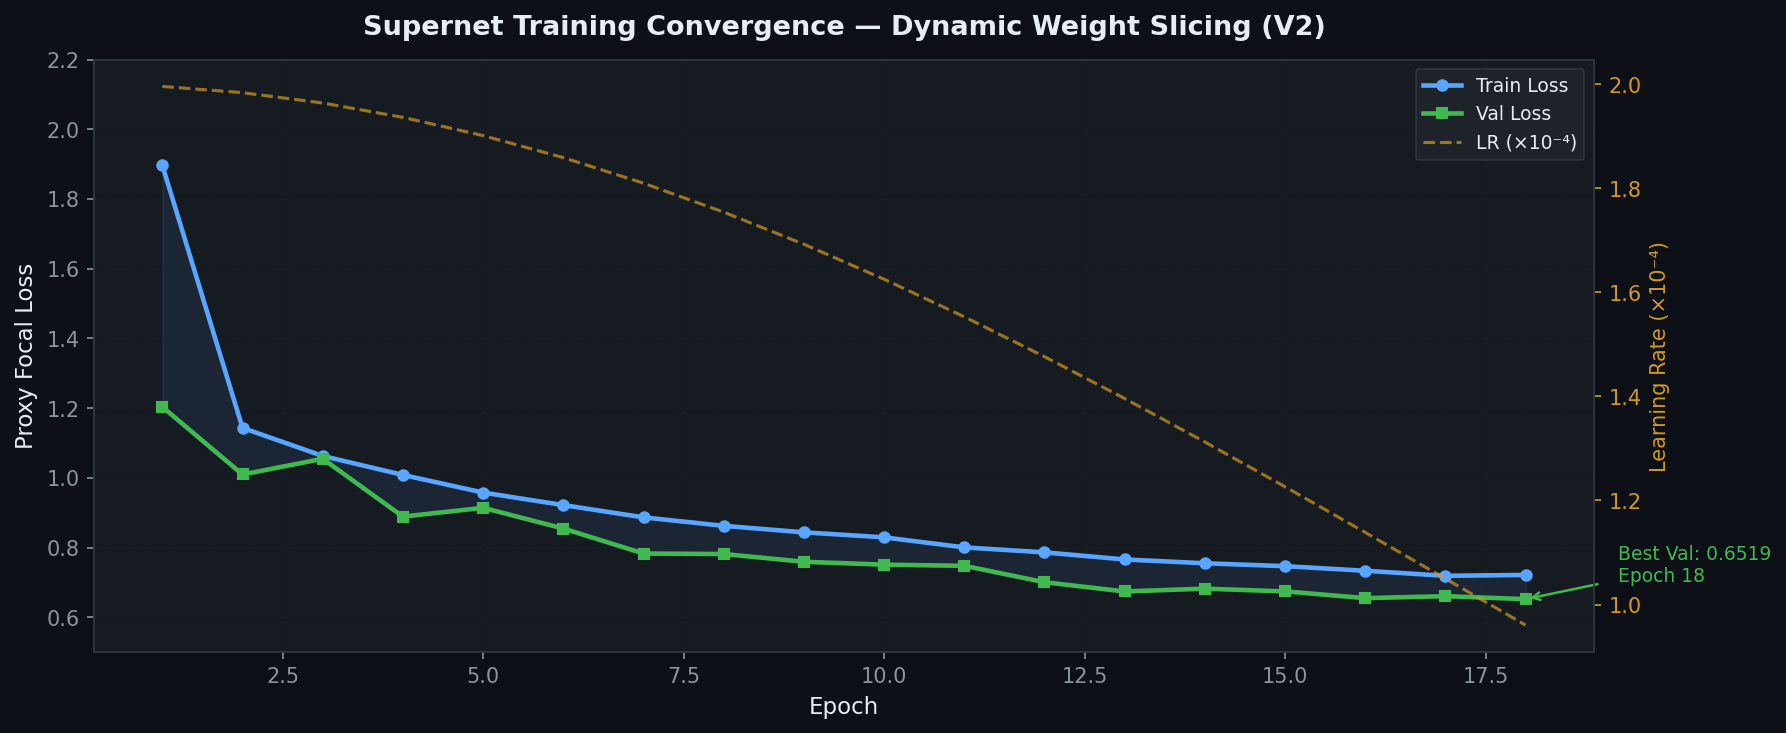
\includegraphics[width=0.98\linewidth,height=0.82\textheight,keepaspectratio]{fig1_training_curve.png}
  \end{figure}
\end{frame}

\begin{frame}{Leaderboard 1,000 Candidate}
  \begin{figure}
    \centering
    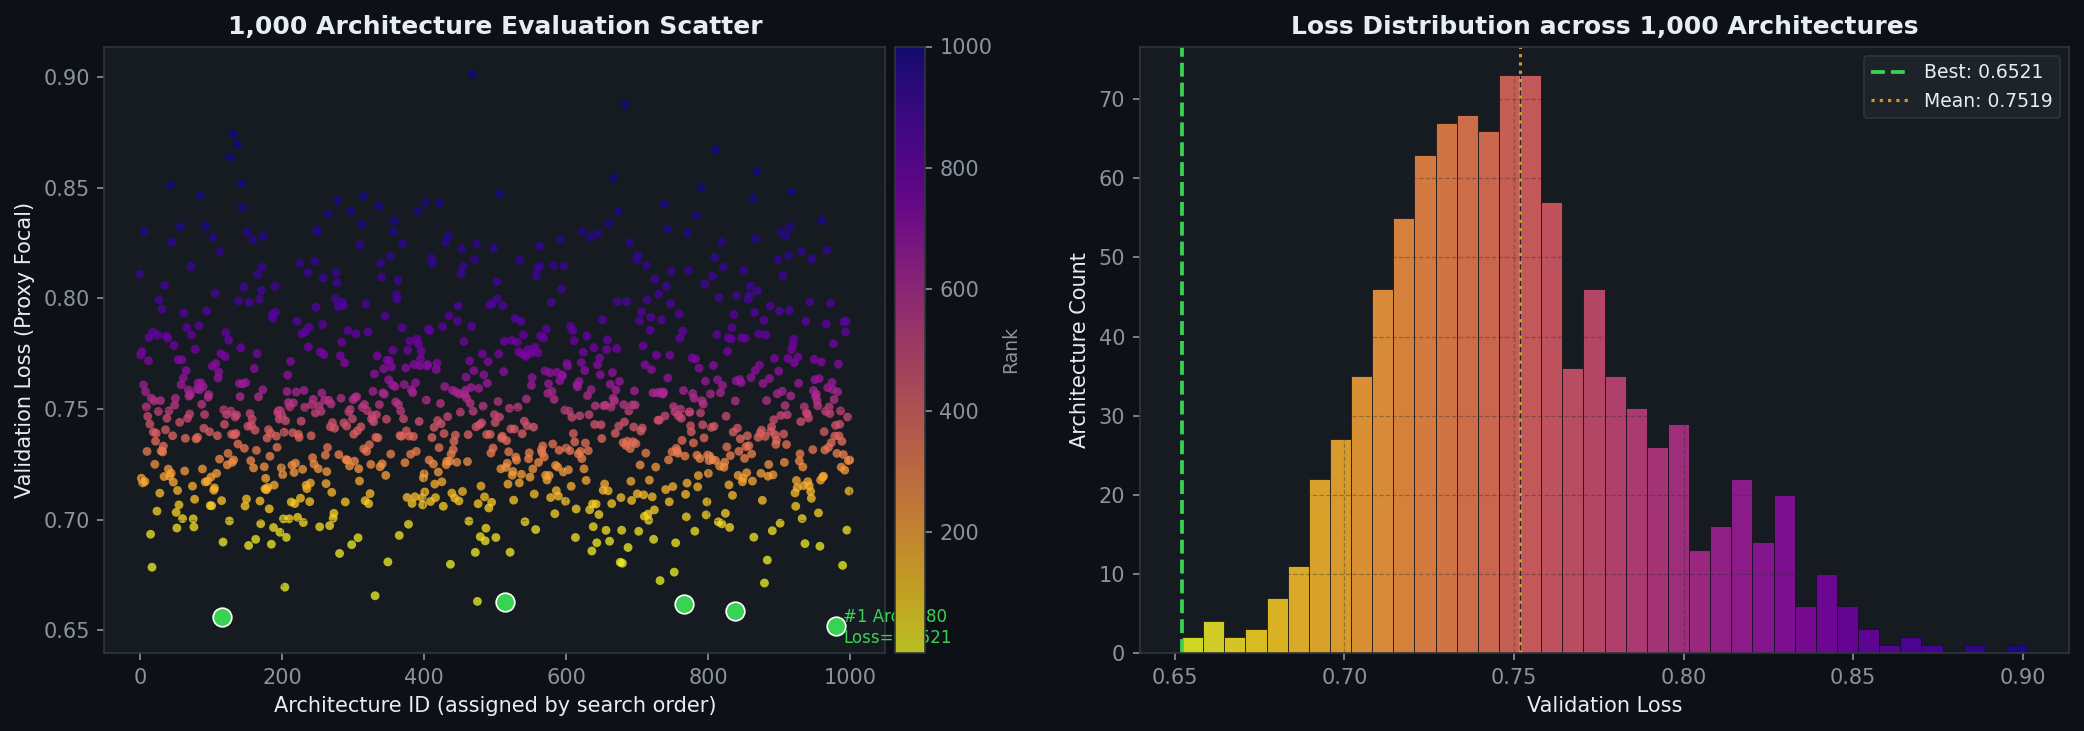
\includegraphics[width=0.98\linewidth,height=0.82\textheight,keepaspectratio]{fig2_nas_leaderboard.png}
  \end{figure}
\end{frame}

\begin{frame}{Kết quả chính của SPOS-NAS}
  \begin{itemize}
    \item Nhóm tốt có xu hướng \textbf{đầu tư mạnh vào \(C_2\)} và tránh làm \(C_3\) phình quá mức.
    \item \(C_2\) giữ chi tiết vị trí không gian cho tiny faces, còn \(C_5\) bổ sung ngữ nghĩa đủ mạnh cho head.
    \item \(C_3\) là vùng dễ thành bẫy chi phí: feature map vẫn còn lớn nên chi phí đắt, nhưng gain tăng không tương xứng.
    \item Khi đổi proxy từ center-focus sang edge-focus, phân bố học dịch chuyển (giảm C2 tăng C3) \(\rightarrow\) phản ứng linh hoạt với hình học của bài toán (vì ở viền cần thêm ngữ cảnh không gian nên cần stride lớn hơn).
  \end{itemize}
\end{frame}

\begin{frame}{Phân tích cơ cấu phân bố: Tránh bẫy FLOPs ở C3}
  \begin{figure}
    \centering
    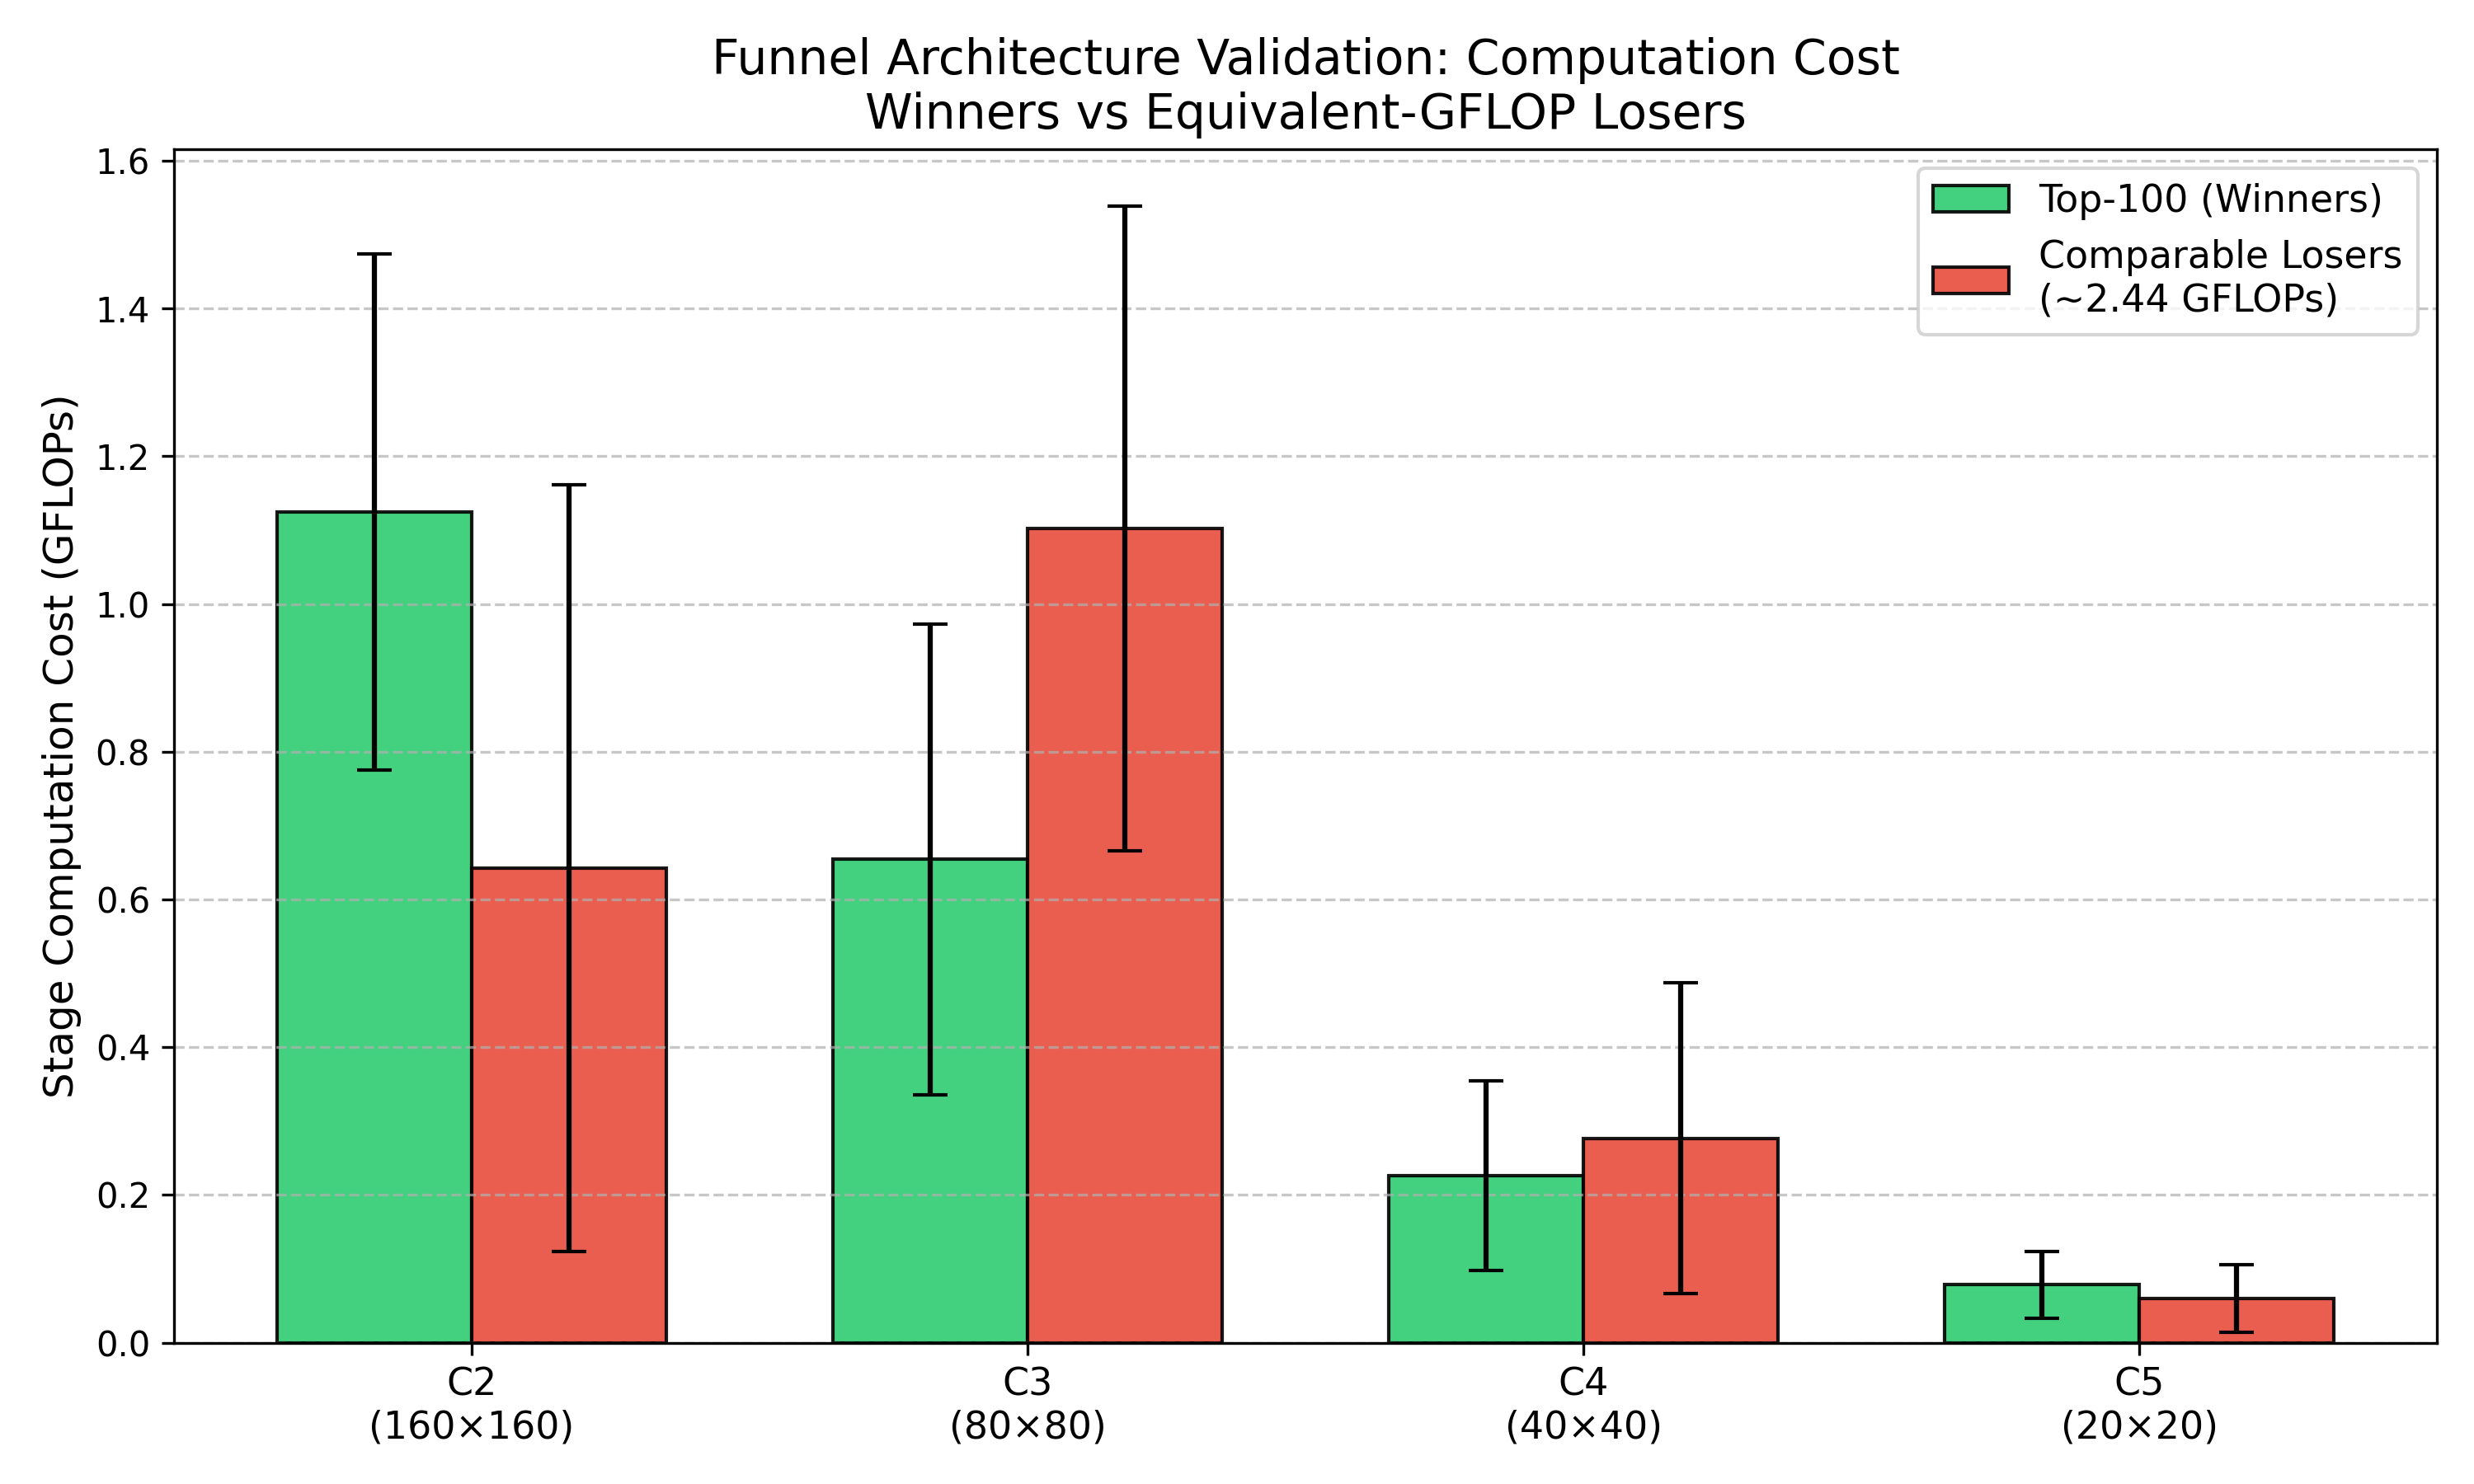
\includegraphics[width=0.98\linewidth,height=0.82\textheight,keepaspectratio]{fig3_funnel_analysis.png}
  \end{figure}
\end{frame}

\begin{frame}{Top winners dành compute cho C2 và C5}
  \begin{figure}
    \centering
    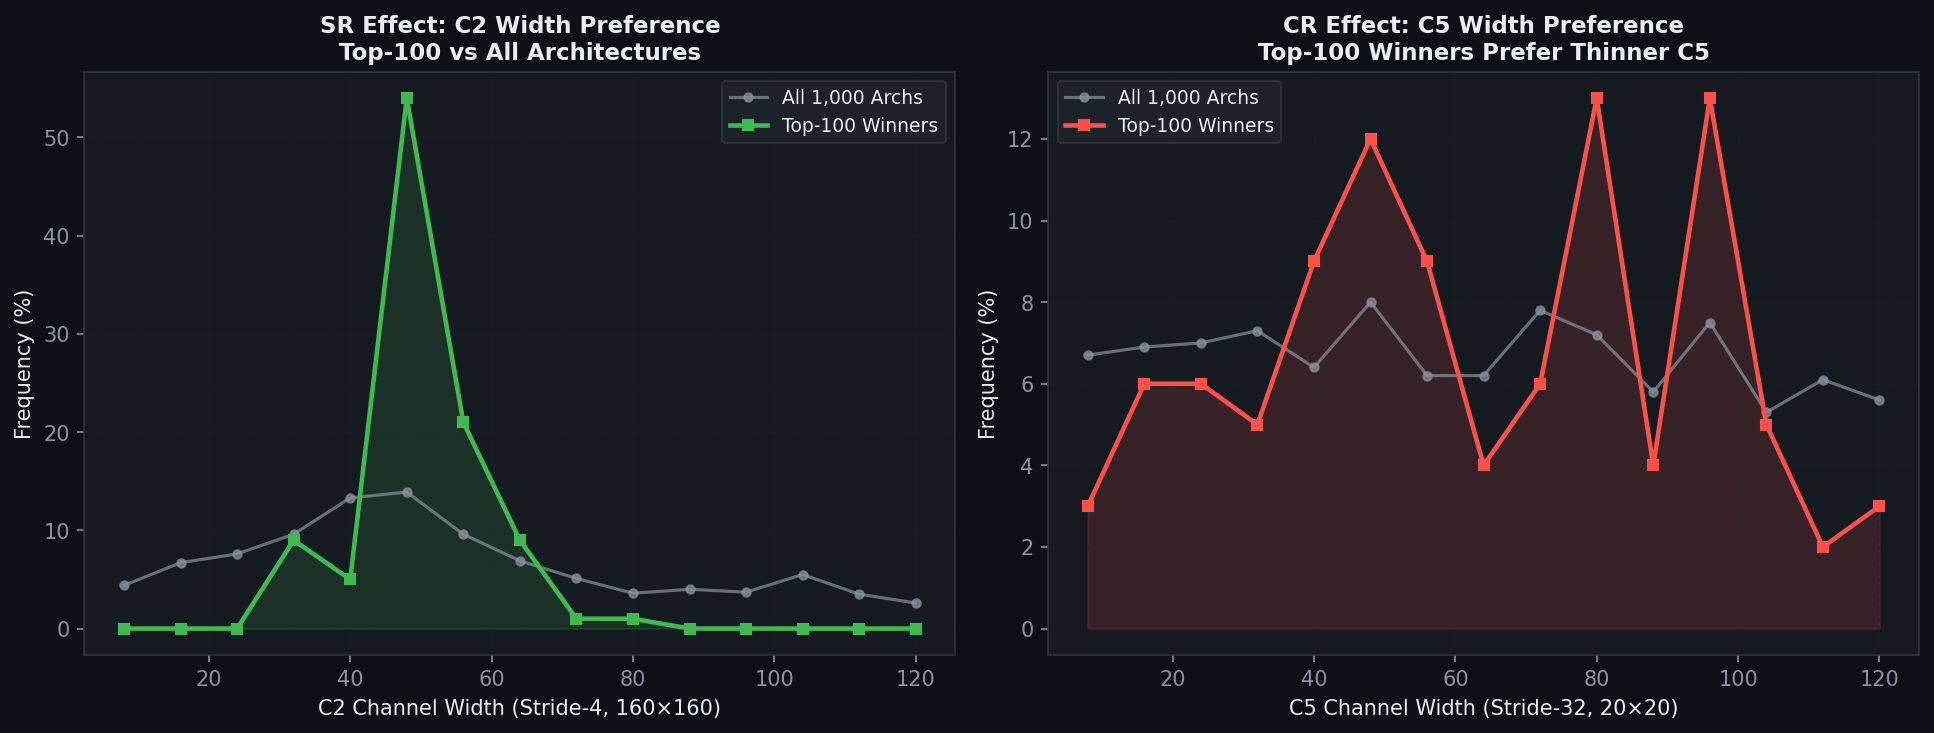
\includegraphics[width=0.98\linewidth,height=0.82\textheight,keepaspectratio]{fig5_c2_c5_distributions.png}
  \end{figure}
\end{frame}

\begin{frame}{Phân tích cơ cấu phân bố: Tập trung vào biên (Edge-focus)}
  \begin{figure}
    \centering
    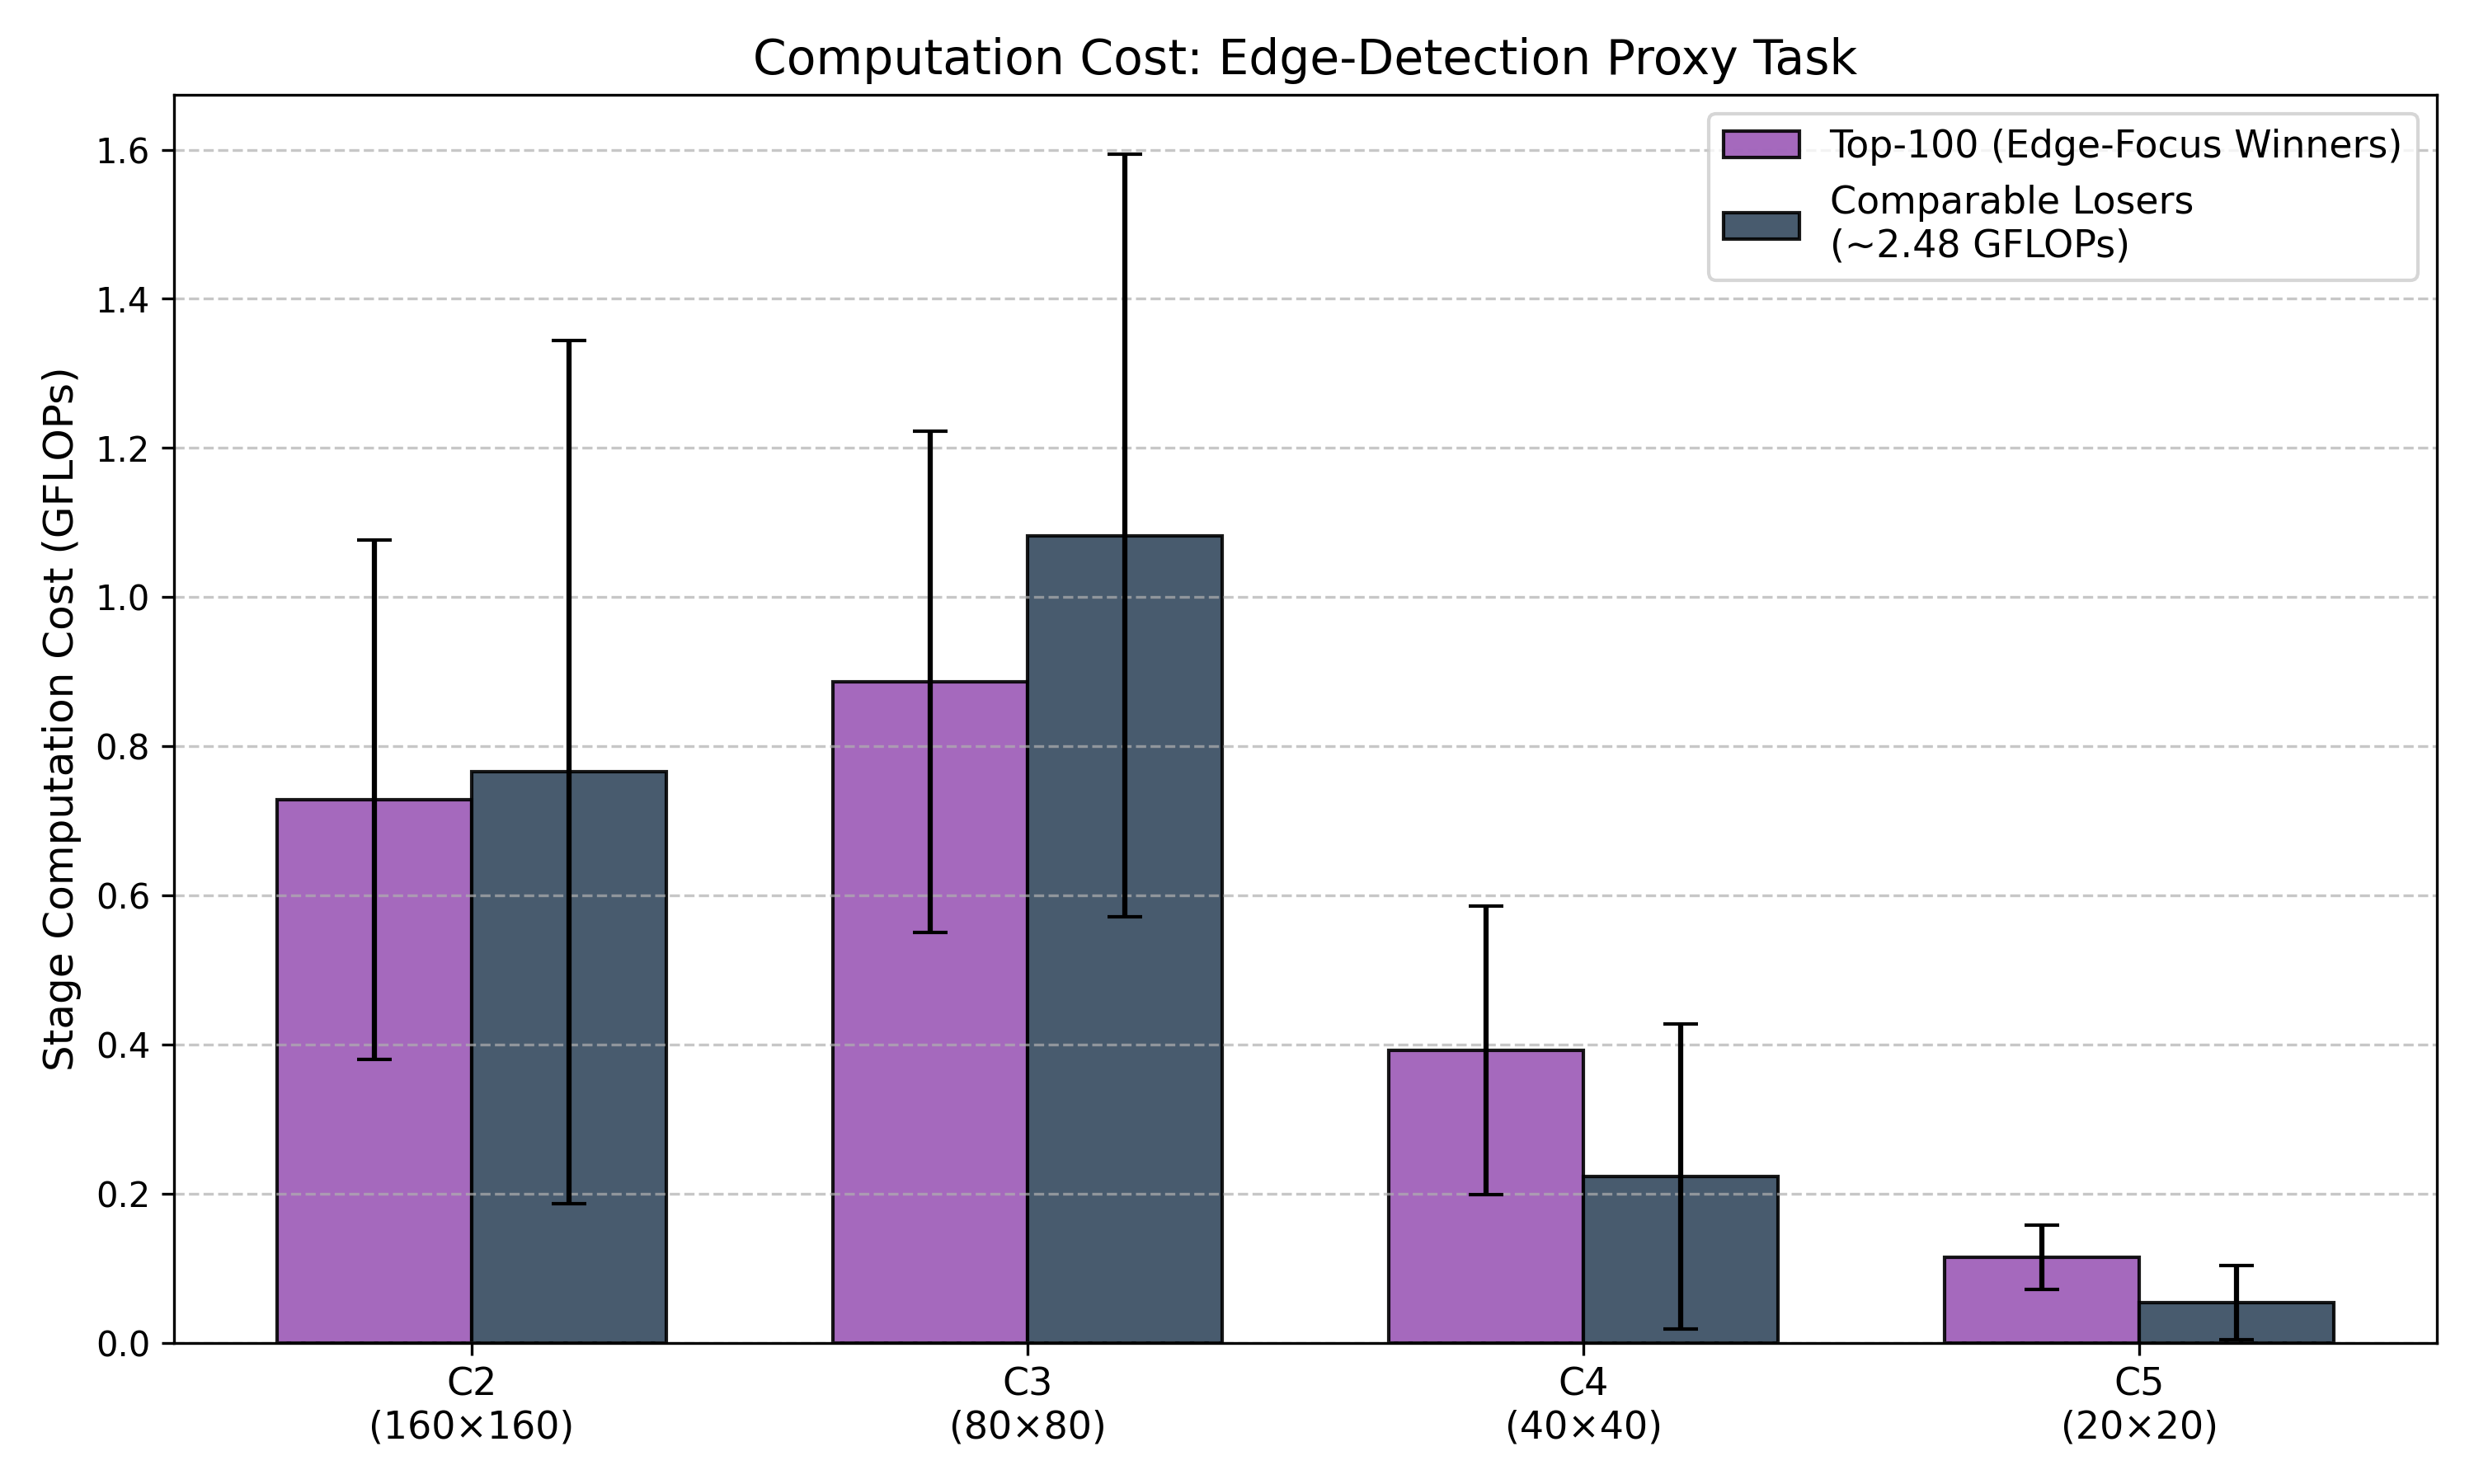
\includegraphics[width=0.98\linewidth,height=0.82\textheight,keepaspectratio]{fig_appendix_edge_funnel.png}
  \end{figure}
\end{frame}

\begin{frame}{Insight chốt lại từ SPOS-NAS}
  \begin{block}{Điểm mà phần mở rộng này xác nhận}
    Computation Redistribution của SCRFD là một nguyên tắc phân bổ compute có cấu trúc, không phải mẹo thử-sai ngẫu nhiên.
  \end{block}
  \begin{itemize}
    \item Trong miền 2.5 GFLOPs, winner thắng vì phân bổ compute đúng hơn, không phải vì đơn giản lớn hơn.
    \item Đó là lý do report kết luận SCRFD mạnh vì nó đặt năng lực biểu diễn đúng chỗ ngay từ cấp kiến trúc.
  \end{itemize}
\end{frame}

\section{ASR+JSAR: Điều chỉnh tỉ lệ cắt và gán mẫu khi huấn luyện}

\begin{frame}{Động cơ của ASR+JSAR}
  \small
  \textbf{Adaptive Sample Redistribution (ASR)} và \textbf{Joint Sample Assignment Redistribution (JSAR)}
  là hai cải tiến được thêm vào giai đoạn huấn luyện của SCRFD.
  \vspace{0.4em}
  \begin{itemize}
    \item Sau baseline dùng bộ 12 mức theo bài báo, gap lớn nhất vẫn nằm ở split Hard.
    \item Điều đó cho thấy phân phối chọn tỉ lệ cắt tĩnh vẫn chưa đủ, và tiny faces vẫn còn bị thiếu mẫu dương ở bước gán nhãn.
    \item Vì vậy nhóm sửa đúng hai nút thắt của giai đoạn train:
  \end{itemize}
  \begin{block}{Hai cải tiến}
    \textbf{Adaptive Sample Redistribution (ASR)}: điều chỉnh động xác suất chọn các mức tỉ lệ cắt khi tăng cường dữ liệu theo tín hiệu khó dễ đang quan sát được.\\
    \textbf{Joint Sample Assignment Redistribution (JSAR)}: tăng số mẫu dương được gán cho tiny faces khi quy tắc gán chuẩn còn bỏ sót.
  \end{block}
  \vfill
  {\tiny
  Nguồn tham khảo: ý tưởng được tham khảo từ \textbf{Sample Redistribution} của SCRFD~\cite{guo2022scrfd}
  và \textbf{ATSS} cho bước gán mẫu~\cite{zhang2020atss}.}
\end{frame}

\begin{frame}{Cấu hình huấn luyện của ASR+JSAR}
  \scriptsize
  \begin{columns}[T,onlytextwidth]
    \column{0.48\textwidth}
    \begin{block}{Thiết lập chung}
      \begin{itemize}
        \item Mô hình: \textbf{SCRFD-2.5GF}, input \(640\times640\)
        \item Số epoch: \textbf{80}
        \item Phần cứng: \textbf{1 $\times$ NVIDIA RTX 3090}
        \item Batch size: \textbf{32}
        \item Optimizer: \textbf{SGD}, momentum \(=0.9\), weight decay \(=5\times10^{-4}\)
        \item Learning rate ban đầu: \textbf{0.04}
        \item Lịch học: \textbf{CosineAnnealing}, warmup tuyến tính 1500 iter, warmup ratio \(=10^{-3}\), min lr \(=0\)
      \end{itemize}
    \end{block}
    \column{0.48\textwidth}
    \begin{block}{Tham số ASR và JSAR}
      \begin{itemize}
        \item ASR: warmup \(=2\) epoch, update interval \(=1000\), EMA \(=0.8\), min prob \(=0.03\)
        \item Bin kích thước: \([0,16), [16,32), [32,96), [96,+\infty)\)
        \item Tiny / small threshold: \(16\) và \(32\)
        \item IoU delta: tiny \(=0.05\), small \(=0.02\)
        \item Top-k \(=4\), center radius scale \(=1.3\)
        \item Min positive / tiny GT \(=3\)
      \end{itemize}
    \end{block}
  \end{columns}
  \vspace{0.05cm}
  Bộ tỉ lệ cắt của ASR thay đổi theo thí nghiệm: bộ mặc định hoặc bộ 12 mức theo bài báo.
\end{frame}

\begin{frame}{ASR và JSAR hoạt động như thế nào}
  \begin{columns}[T,onlytextwidth]
    \column{0.49\textwidth}
    \begin{block}{ASR}
      \begin{itemize}
        \item Bắt đầu từ một bộ ứng viên tỉ lệ cắt đủ rộng.
        \item Gom thống kê face-size distribution và thiếu hụt recall theo từng giai đoạn train.
        \item Điều chỉnh xác suất chọn các mức tỉ lệ cắt để tăng tần suất xuất hiện của nhóm tiny/small faces còn thiếu.
        \item Làm mượt phân phối xác suất bằng EMA để tránh dao động quá mạnh.
      \end{itemize}
    \end{block}
    \column{0.49\textwidth}
    \begin{block}{JSAR}
      \begin{itemize}
        \item Tiny faces thường nhận quá ít mẫu dương với quy tắc gán gốc.
        \item JSAR nới lỏng bước chọn ứng viên quanh tâm.
        \item Nếu vẫn thiếu mẫu dương, fallback sẽ giữ lại một nhóm anchor gần nhất còn hợp lý.
        \item Nhờ đó tiny faces không còn bị rơi khỏi supervision.
      \end{itemize}
    \end{block}
  \end{columns}
\end{frame}

\begin{frame}{ASR: công thức điều chỉnh phân phối tỉ lệ cắt}
  \small
  \begin{columns}[T,onlytextwidth]
    \column{0.52\textwidth}
    \begin{block}{Đo độ khó theo từng nhóm kích thước}
    \[
      r_b=\max\!\left(0,\;1-\min\!\left(\frac{P_b}{\max(G_b,1)},1\right)\right)
    \]
    \[
      c_b=\frac{L^{cls}_b}{\max(P_b,1)},\qquad
      u_b=\frac{L^{box}_b}{\max(P_b,1)}
    \]
    \[
      d_b \propto \mathrm{norm}(r_b)+\mathrm{norm}(c_b)+\mathrm{norm}(u_b)
    \]
    \end{block}
    \column{0.46\textwidth}
    \begin{block}{Cập nhật xác suất chọn tỉ lệ cắt}
    \[
      q(s)=\sum_b M(s,b)\,d_b
    \]
    \[
      \hat p(s)=\frac{q(s)}{\sum_j q(j)}
    \]
    \[
      p_{t+1}(s)=\alpha p_t(s)+(1-\alpha)\,\mathrm{floor}(\hat p(s))
    \]
    \end{block}
  \end{columns}

  \vspace{0.15cm}
  \begin{itemize}
    \item \(b\): nhóm kích thước mặt; \(s\): tỉ lệ cắt ảnh; \(M(s,b)\): mức hỗ trợ giữa mỗi mức cắt và từng nhóm kích thước.
    \item ASR tăng xác suất cho các mức tỉ lệ cắt tạo ra nhiều tín hiệu học hơn ở các nhóm còn khó.
    \item Tỉ lệ cắt nhỏ tương ứng \textbf{zoom-in}; tỉ lệ cắt lớn tương ứng \textbf{zoom-out}.
  \end{itemize}
\end{frame}

\begin{frame}{JSAR: công thức nới phép gán mẫu cho tiny faces}
  \small
  \begin{columns}[T,onlytextwidth]
    \column{0.50\textwidth}
    \begin{block}{Hạ ngưỡng và nới center gating}
    \[
      \tau'_g=\tau_g-\Delta_g,\qquad
      \Delta_g=
      \begin{cases}
        0.05, & \mathrm{size}_g<16\\
        0.02, & 16\le \mathrm{size}_g<32\\
        0, & \text{otherwise}
      \end{cases}
    \]
    \[
      c_g=\mathrm{clip}\!\left(\frac{\mathrm{size}_g}{T_{tiny}},1,\rho\right)
    \]
    \[
      \text{keep if }\mathrm{dist}_{\min}(a,g)\,c_g > t_{center}
    \]
    \end{block}
    \column{0.48\textwidth}
    \begin{block}{Fallback top-k nếu vẫn thiếu mẫu dương}
    \[
      \mathrm{score}(a,g)=\mathrm{IoU}(a,g)-0.05\,
      \frac{\mathrm{dist}(a,g)}{\max(\mathrm{size}_g,1)}
    \]
    \[
      \mathcal{P}_g \leftarrow \mathcal{P}_g \cup \mathrm{TopK}(\mathrm{score},k)
    \]
    \[
      |\mathcal{P}_g| \ge N_{\min},\quad N_{\min}=3 \text{ cho tiny GT}
    \]
    \end{block}
  \end{columns}

  \vspace{0.15cm}
  \begin{itemize}
    \item JSAR chỉ can thiệp mạnh vào tiny/small faces; medium và large gần như giữ nguyên.
    \item Ý nghĩa chính: tiny faces không còn bị rơi khỏi supervision chỉ vì IoU thấp hoặc center constraint quá chặt.
  \end{itemize}
\end{frame}

\begin{frame}{ASR: hình học của bộ tỉ lệ cắt}
  \begin{figure}
    \centering
    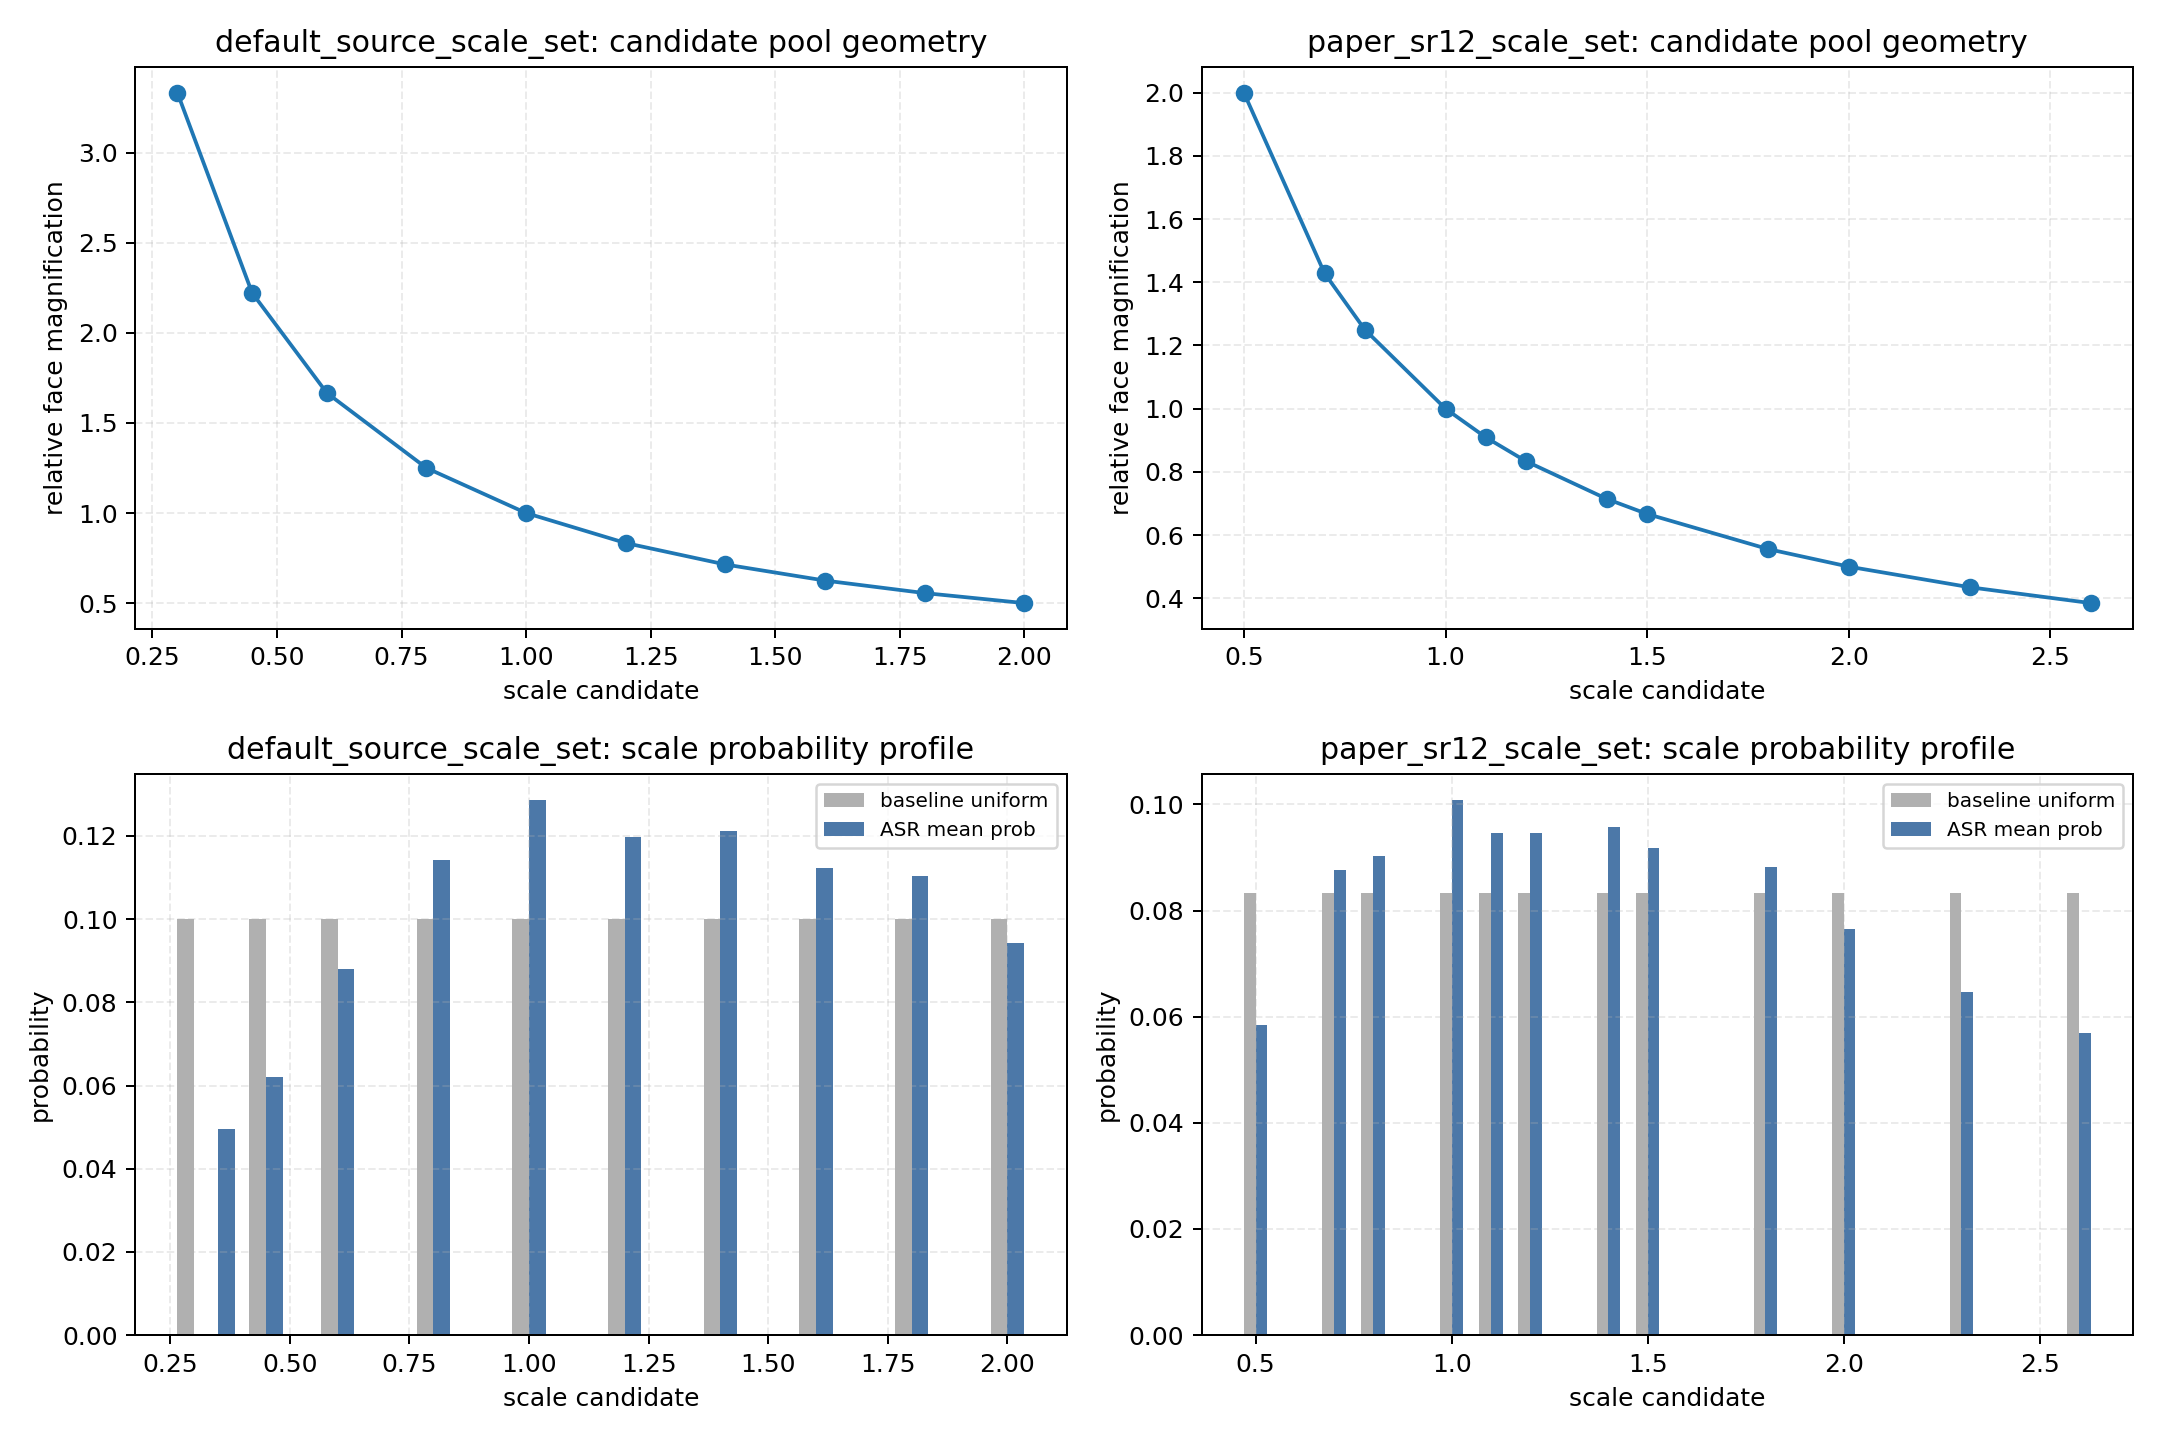
\includegraphics[width=0.93\linewidth,height=0.72\textheight,keepaspectratio]{../../figures/final_term_spos_scrfd/scale_pool_geometry.png}
  \end{figure}
  \vspace{-0.15cm}
  \footnotesize
  \begin{itemize}
    \item Tỉ lệ cắt nhỏ làm khuôn mặt lớn hơn sau resize; tỉ lệ cắt lớn làm khuôn mặt nhỏ hơn sau resize.
  \end{itemize}
\end{frame}

\begin{frame}{ASR: áp lực phân phối theo nhóm kích thước}
  \begin{figure}
    \centering
    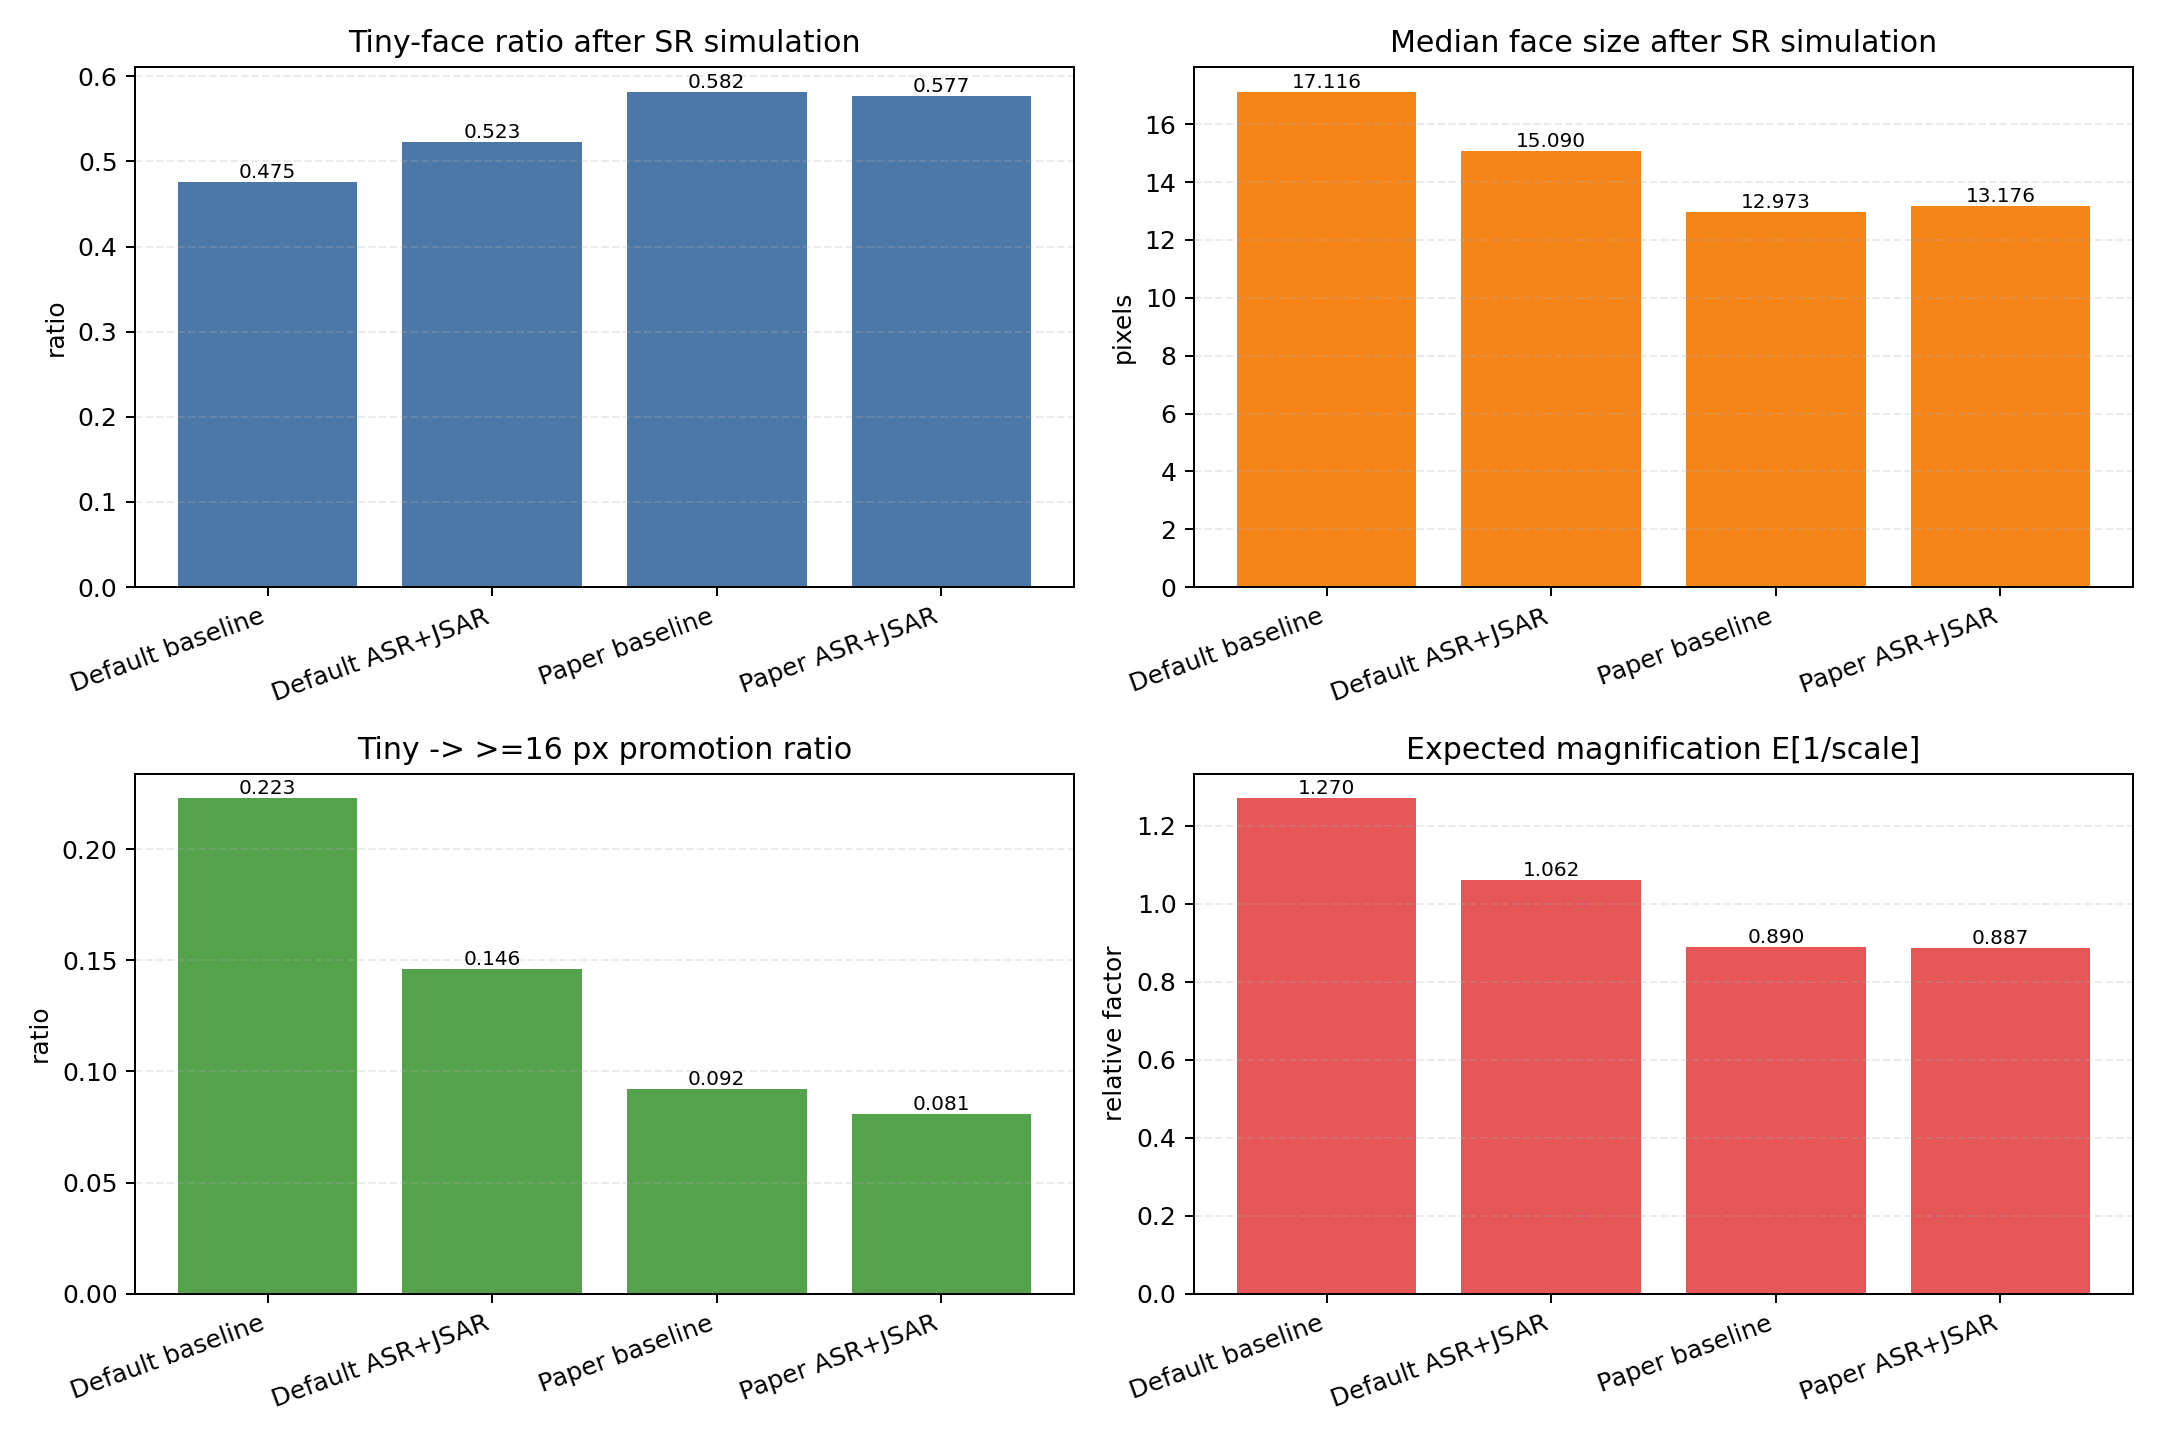
\includegraphics[width=0.93\linewidth,height=0.72\textheight,keepaspectratio]{../../figures/final_term_spos_scrfd/distribution_pressure.png}
  \end{figure}
  \vspace{-0.15cm}
  \footnotesize
  \begin{itemize}
    \item Khi một nhóm kích thước còn khó, ASR sẽ tăng xác suất cho các mức tỉ lệ cắt có khả năng tạo thêm tín hiệu học cho đúng nhóm đó.
  \end{itemize}
\end{frame}

\begin{frame}{Protocol thực nghiệm cho ASR+JSAR}
  \begin{itemize}
    \item Cả baseline và cải tiến đều dùng \textbf{SCRFD-2.5GF}, input \(640\times640\), 80 epoch, cosine scheduler.
    \item Nhóm chạy hai cặp thí nghiệm để tách ảnh hưởng của bộ tỉ lệ cắt và cơ chế điều chỉnh động trong lúc train:
  \end{itemize}
  \begin{block}{Hai trường hợp}
    \textbf{Bộ mặc định trong mã nguồn}: baseline gốc của source code.\\
    \textbf{Bộ 12 mức theo bài báo}: tập tỉ lệ cắt gần hơn với narrative của paper.
  \end{block}
  \begin{itemize}
    \item Cách so sánh này giúp đọc đúng delta của ASR+JSAR: gain đến từ việc điều chỉnh động xác suất chọn tỉ lệ cắt và cách gán mẫu dương, không chỉ từ việc đổi bộ tỉ lệ cắt.
    \item Trên nhánh \textbf{mặc định}, baseline và ASR không dùng hoàn toàn cùng điểm đầu bên trái của bộ ứng viên; trên nhánh \textbf{12 mức theo bài báo}, cả hai mới thật sự dùng cùng một tập 12 mức.
  \end{itemize}
\end{frame}

\begin{frame}{Kết quả ASR+JSAR trên WIDER FACE}
  \scriptsize
  \resizebox{\textwidth}{!}{%
  \begin{tabular}{@{}lcccc@{}}
    \toprule
    Thiết lập & Easy & Medium & Hard & mAP \\
    \midrule
    Baseline (mặc định) & 91.40 & 89.69 & 72.49 & 84.53 \\
    ASR+JSAR (mặc định) & 90.39 & 89.25 & 76.90 & 85.51 \\
    Baseline (12 mức theo bài báo) & 91.61 & 89.99 & 73.71 & 85.10 \\
    ASR+JSAR (12 mức theo bài báo) & 90.28 & 89.01 & 77.38 & 85.56 \\
    \bottomrule
  \end{tabular}
  }

  \vspace{0.35cm}
  \begin{itemize}
    \item Gain lớn nhất tập trung ở \textbf{Hard}: \(+4.40\) với bộ mặc định và \(+3.67\) với bộ 12 mức theo bài báo.
    \item Trên bộ 12 mức theo bài báo, kết quả chỉ còn cách official model zoo khoảng \(0.49\) điểm ở split khó nhất.
  \end{itemize}
\end{frame}

\begin{frame}{Các chỉ số theo từng bộ tỉ lệ cắt}
  \begin{figure}
    \centering
    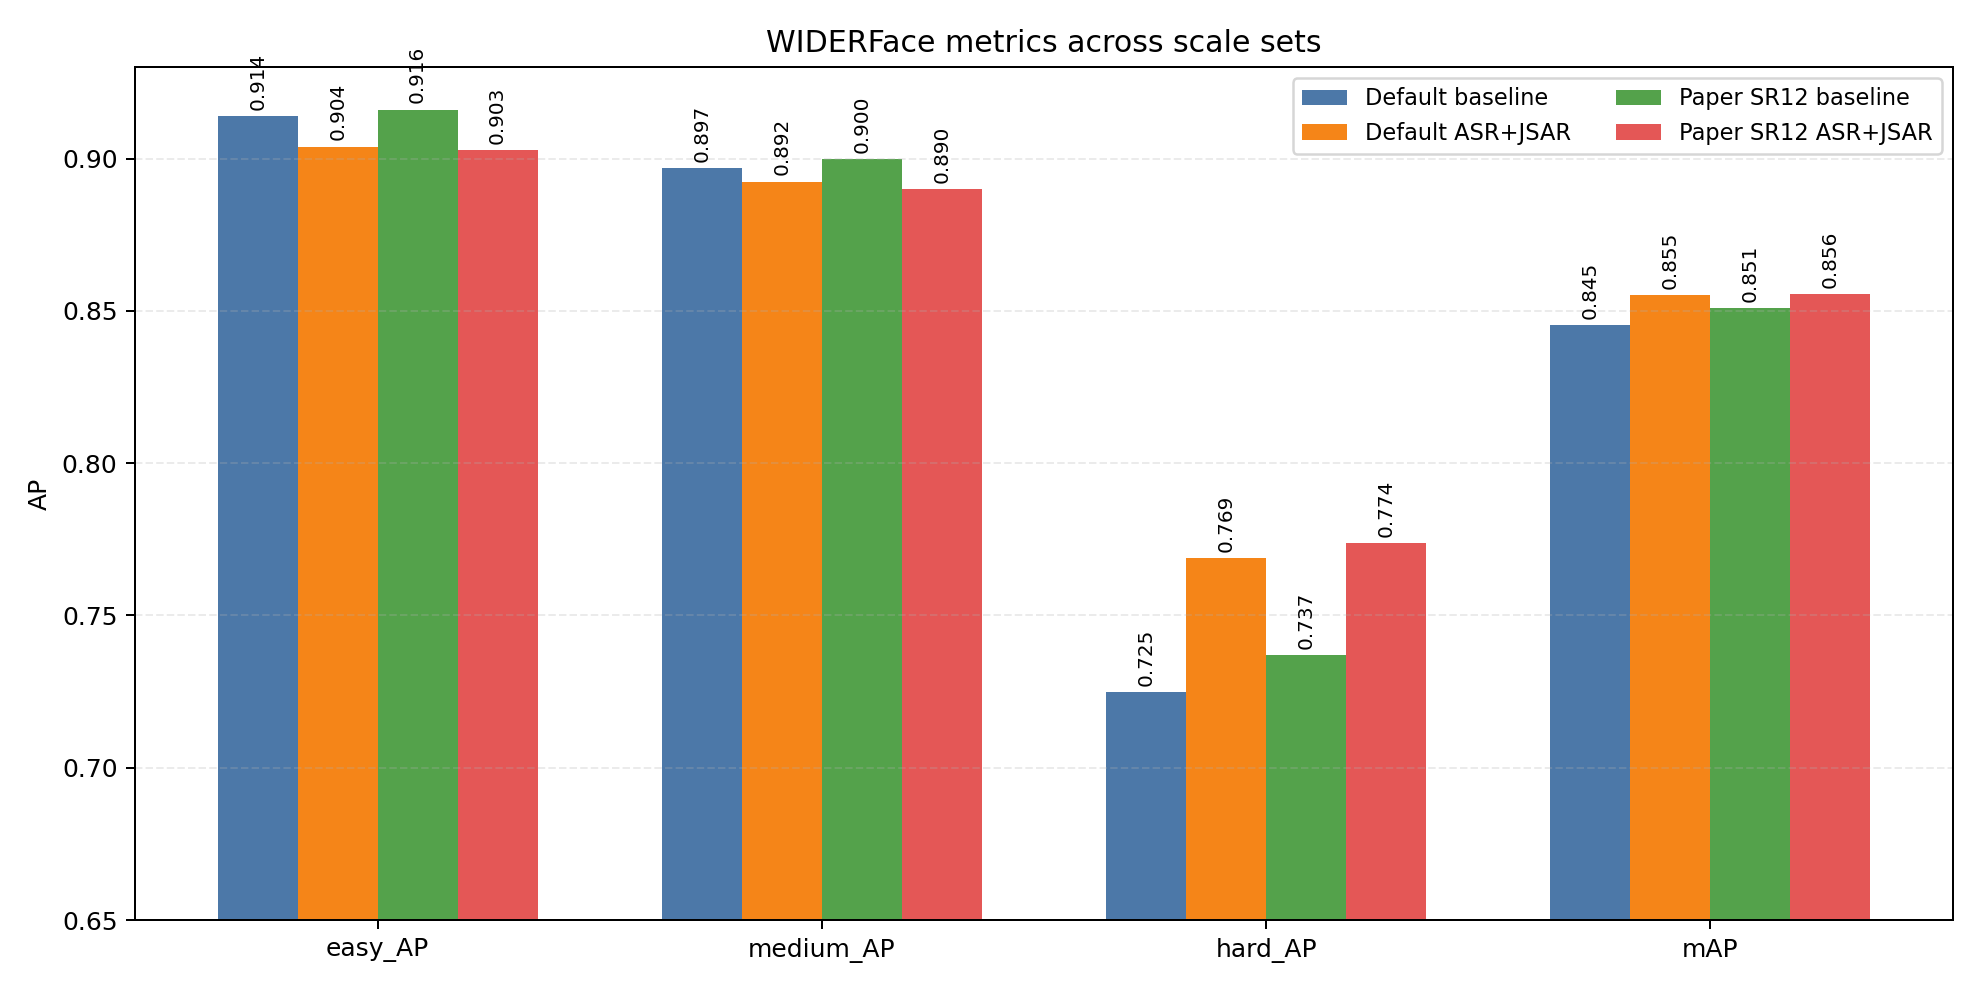
\includegraphics[width=0.94\linewidth,height=0.76\textheight,keepaspectratio]{../../figures/final_term_spos_scrfd/metrics_by_scale_set.png}
  \end{figure}
\end{frame}

\begin{frame}{Delta của ASR+JSAR theo từng bộ tỉ lệ cắt}
  \begin{figure}
    \centering
    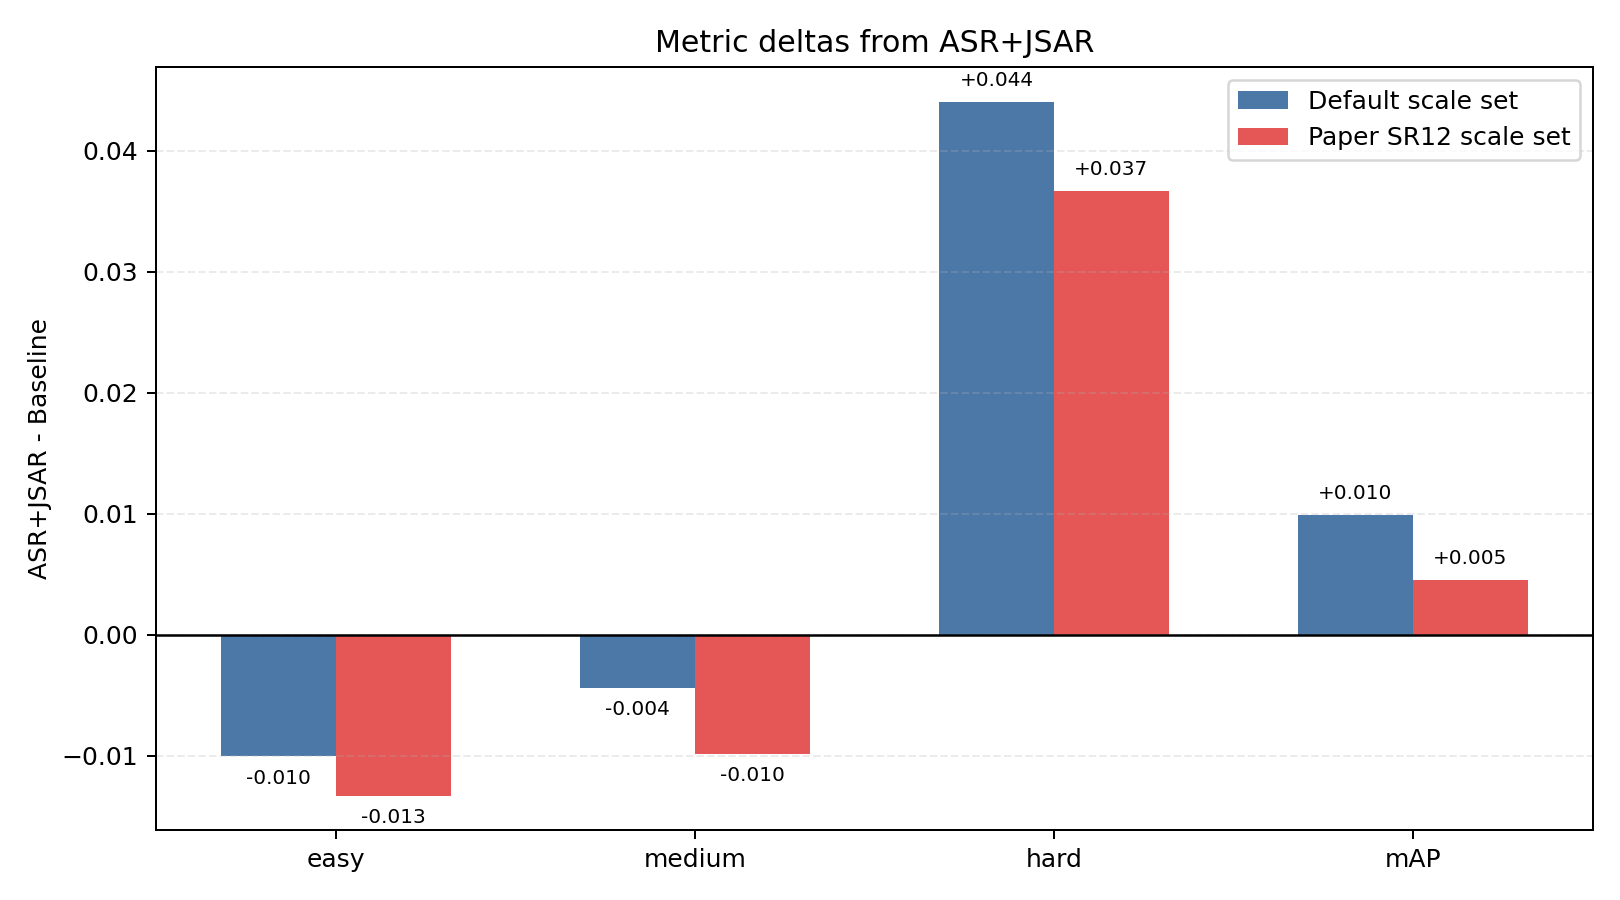
\includegraphics[width=0.94\linewidth,height=0.76\textheight,keepaspectratio]{../../figures/final_term_spos_scrfd/asr_delta_by_scale_set.png}
  \end{figure}
\end{frame}

\begin{frame}{Histogram kích thước khuôn mặt: bộ mặc định trong mã nguồn}
  \begin{figure}
    \centering
    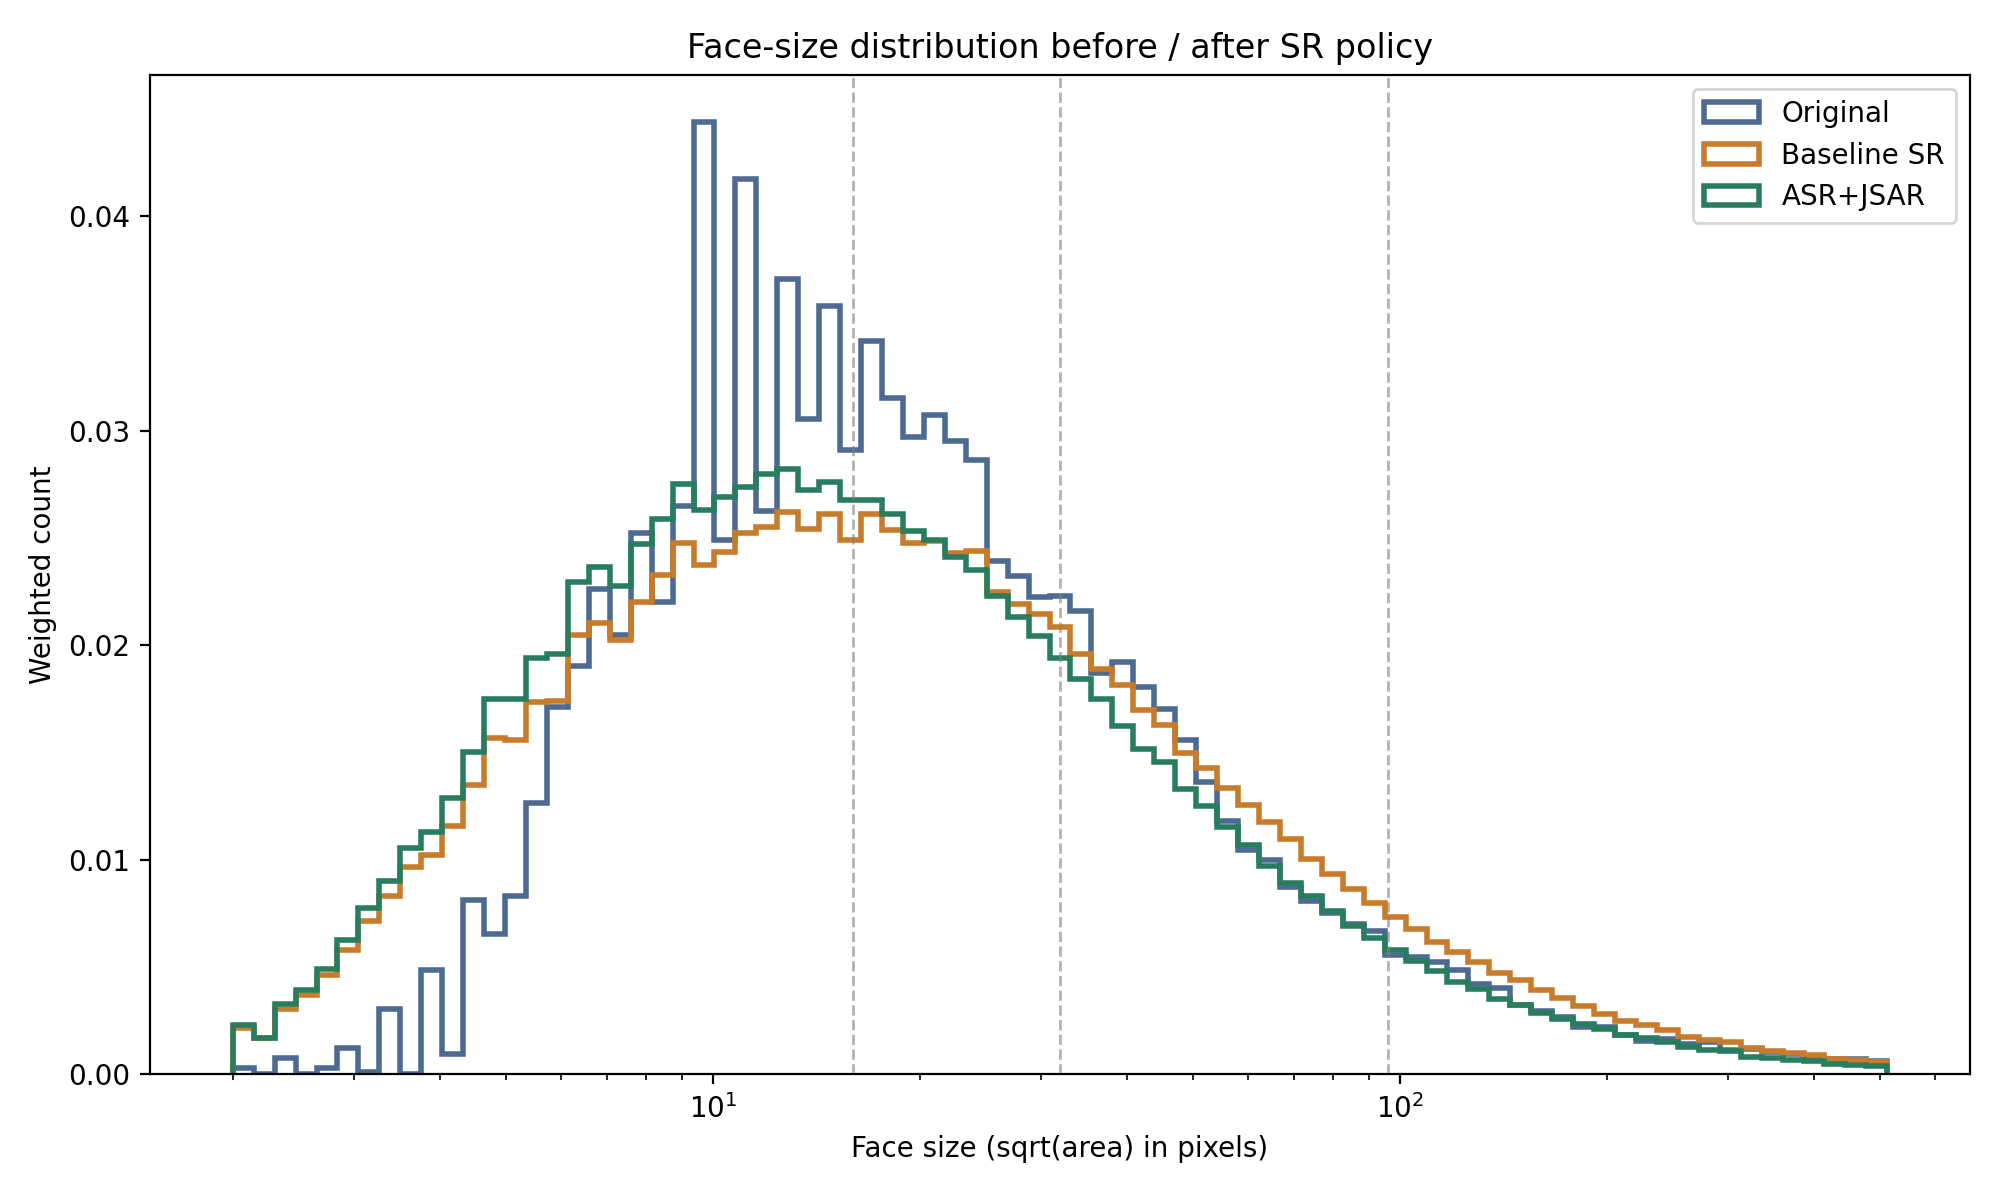
\includegraphics[width=0.94\linewidth,height=0.72\textheight,keepaspectratio]{../../figures/final_term_spos_scrfd/default_face_size_histogram.png}
  \end{figure}
  \vspace{-0.15cm}
  \footnotesize
  \begin{itemize}
    \item Với bộ mặc định, histogram của ASR+JSAR lệch trái rõ hơn baseline, cho thấy mô hình cải tiến chủ động tạo thêm nhiều khuôn mặt nhỏ trong lúc huấn luyện.
  \end{itemize}
\end{frame}

\begin{frame}{Histogram kích thước khuôn mặt: bộ 12 mức theo bài báo}
  \begin{figure}
    \centering
    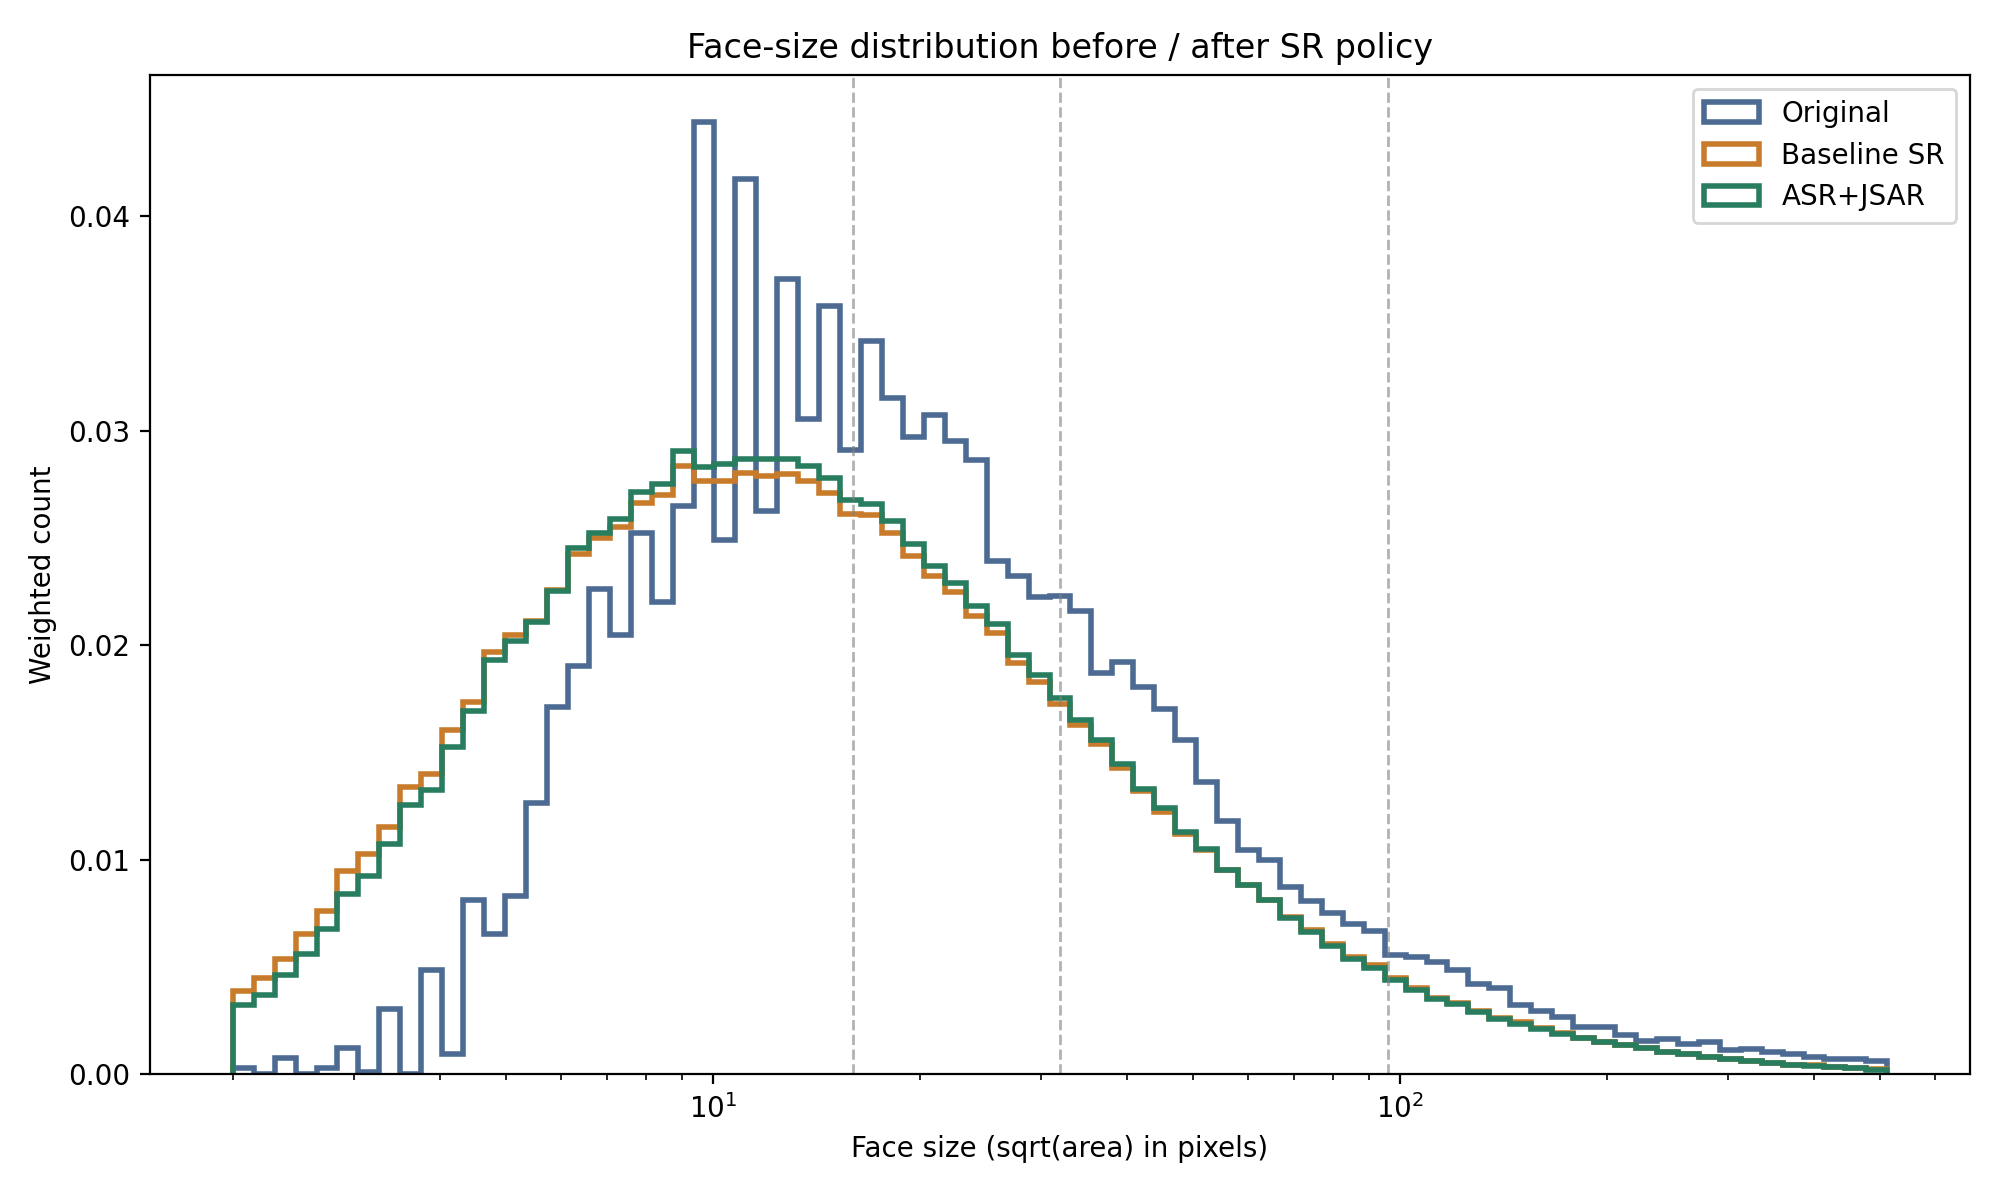
\includegraphics[width=0.94\linewidth,height=0.72\textheight,keepaspectratio]{../../figures/final_term_spos_scrfd/paper_sr12_face_size_histogram.png}
  \end{figure}
  \vspace{-0.15cm}
  \footnotesize
  \begin{itemize}
    \item Với bộ 12 mức theo bài báo, baseline và ASR+JSAR có phân phối gần nhau hơn; phần gain còn lại đến nhiều hơn từ cơ chế gán mẫu của JSAR.
  \end{itemize}
\end{frame}

\begin{frame}{JSAR: mật độ mẫu dương cho tiny faces}
  \begin{figure}
    \centering
    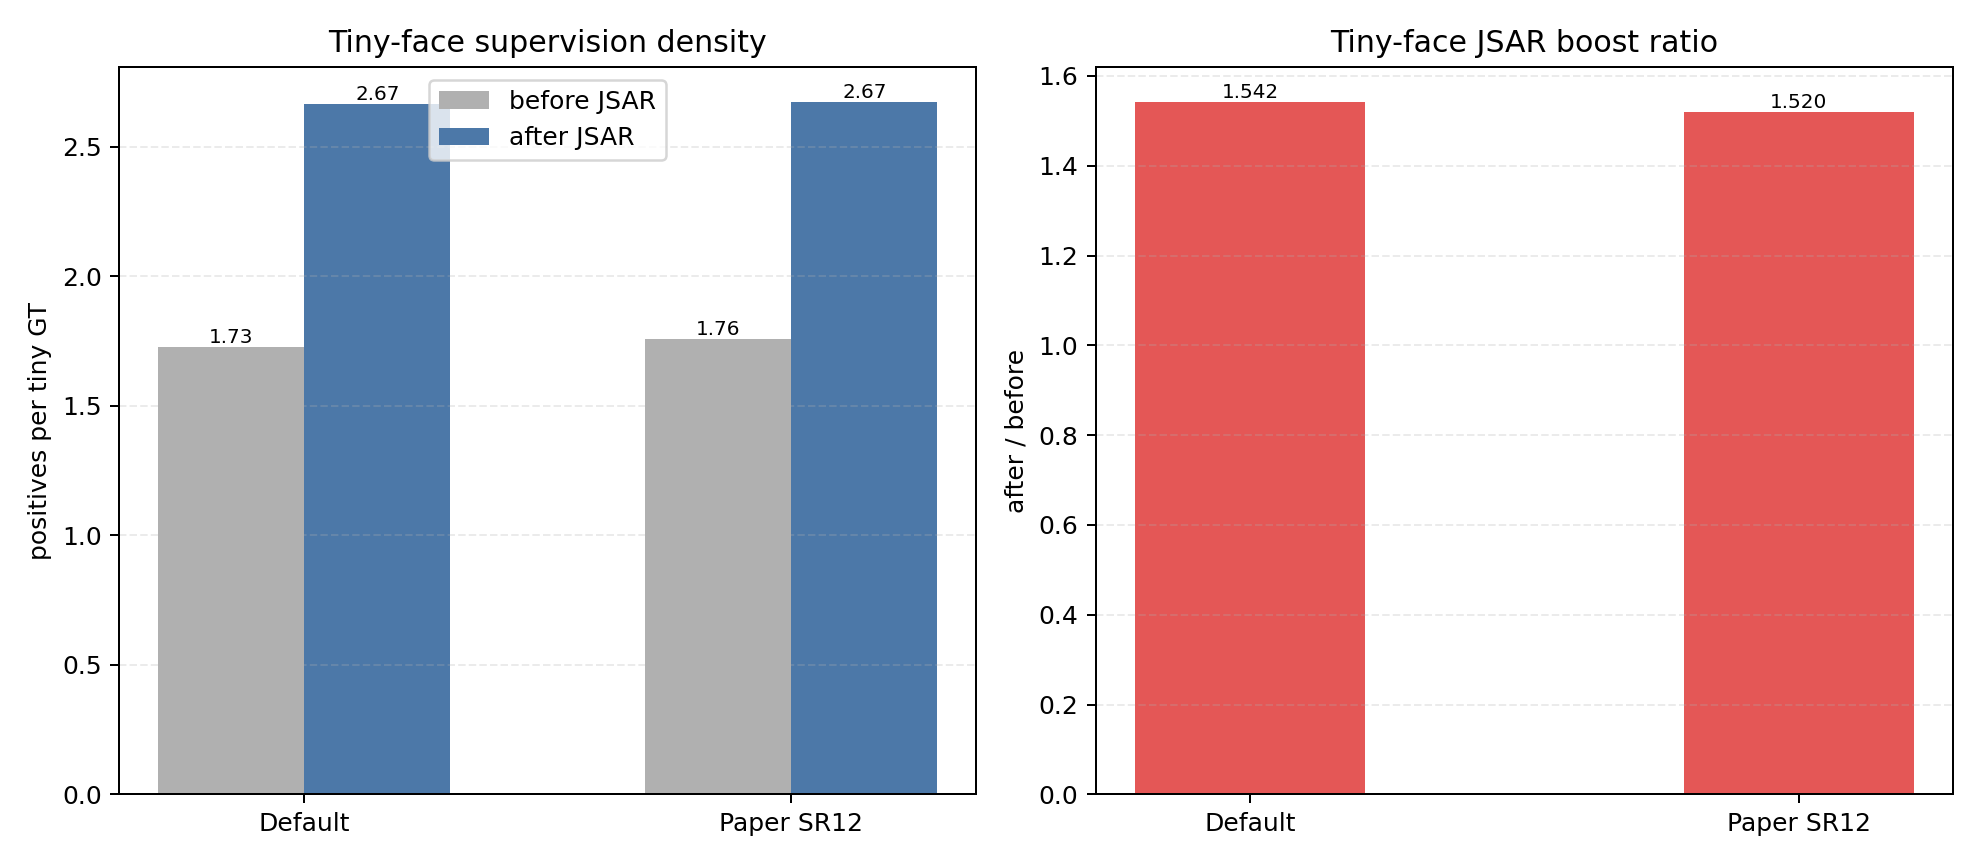
\includegraphics[width=0.94\linewidth,height=0.76\textheight,keepaspectratio]{../../figures/final_term_spos_scrfd/jsar_tiny_supervision.png}
  \end{figure}
\end{frame}

\begin{frame}{Gain theo nhóm khuôn mặt khó}
  \begin{figure}
    \centering
    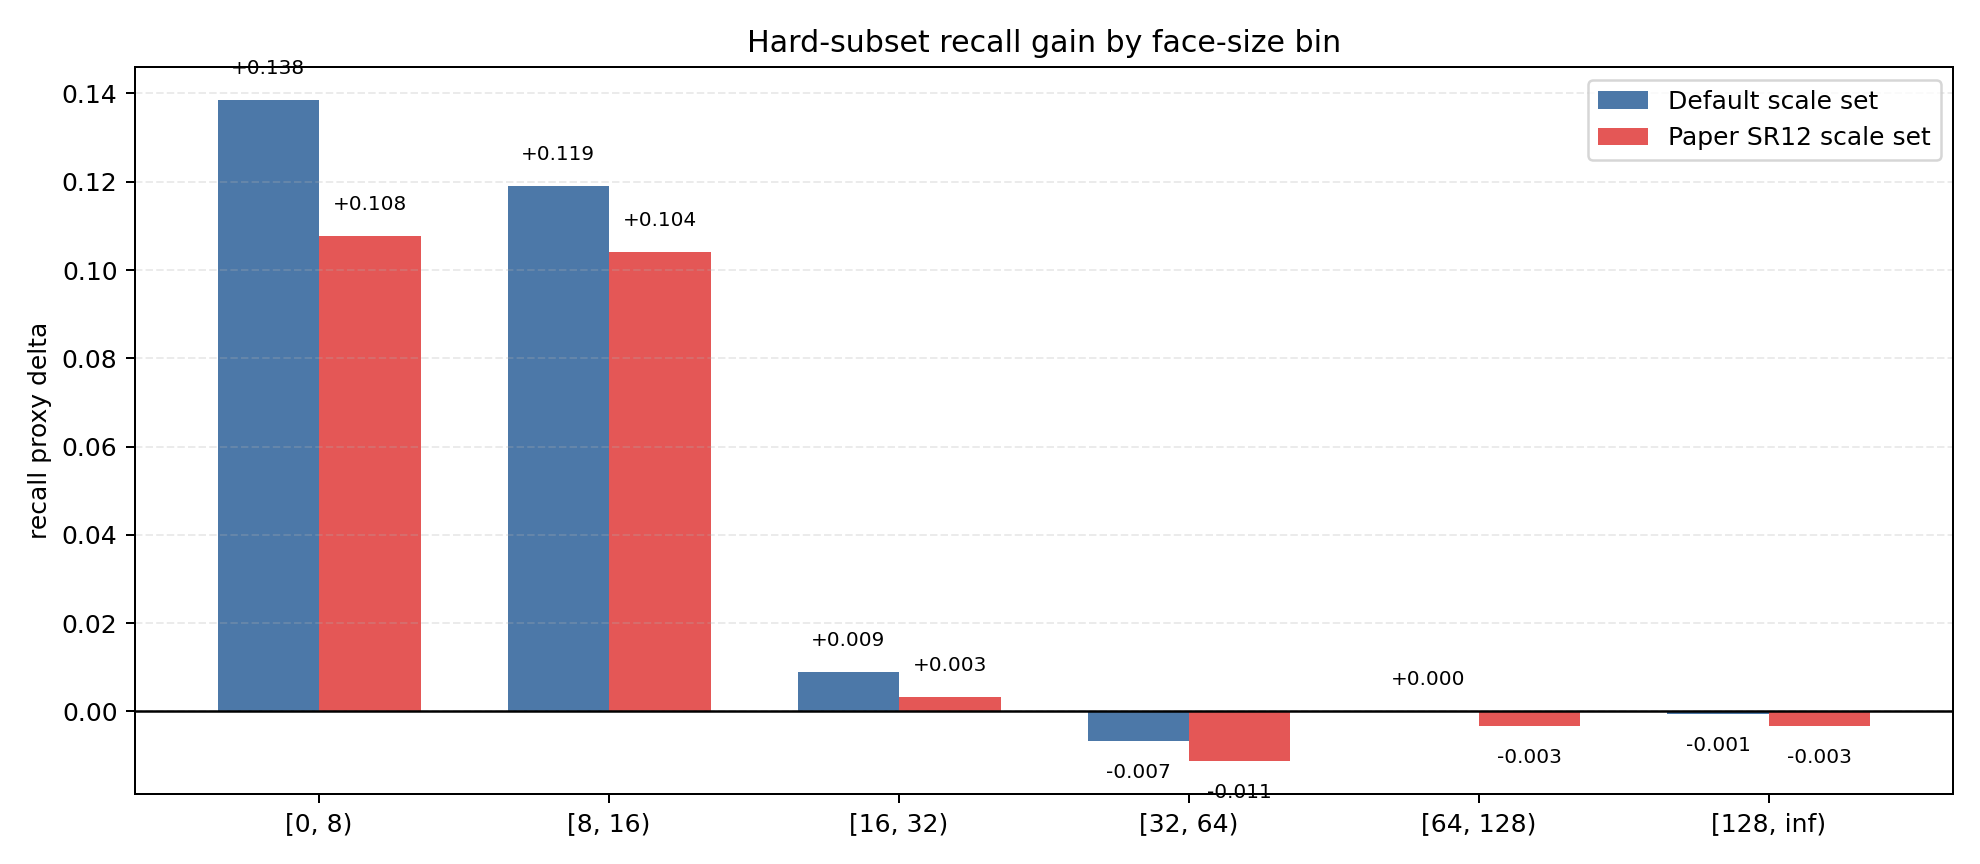
\includegraphics[width=0.94\linewidth,height=0.76\textheight,keepaspectratio]{../../figures/final_term_spos_scrfd/hard_size_gain_by_scale_set.png}
  \end{figure}
\end{frame}

\begin{frame}{Hạn chế}
  \begin{itemize}
    \item Kết quả hiện tại mới được đánh giá trong thiết lập huấn luyện 80 epoch, trong khi bản SCRFD gốc trong bài báo được huấn luyện dài hơn, tới 640 epoch. Vì vậy, chưa thể kết luận đây là mức trần hiệu quả của ASR+JSAR.
    \item Lợi ích của phương pháp tập trung rõ nhất ở khuôn mặt nhỏ và các mẫu thuộc split Hard; đây cũng là nơi SCRFD baseline yếu nhất.
    \item Đổi lại, khi tín hiệu học được dồn nhiều hơn về nhóm khó, hiệu năng trên khuôn mặt vừa và lớn có thể giảm nhẹ. Nói cách khác, cải tiến này không làm tốt đồng đều mọi nhóm kích thước, mà ưu tiên mạnh hơn cho nhóm khó nhất.
  \end{itemize}
\end{frame}

\section{Kết luận}

\begin{frame}{Kết luận}
  \begin{itemize}
    \item SCRFD mạnh vì tối ưu đồng thời \textbf{nơi mô hình đặt năng lực biểu diễn} và \textbf{nơi dữ liệu tạo tín hiệu học}.
    \item \textbf{Baseline reproduction} cho thấy gap lớn nhất luôn nằm ở Hard; đó mới là vùng khó thật của SCRFD.
    \item \textbf{ASR+JSAR} là bằng chứng mạnh nhất của report: giữ nguyên kiến trúc suy luận vẫn có thể kéo Hard AP từ \(73.71\) lên \(77.38\) nếu phân phối tỉ lệ cắt và mật độ mẫu dương cho tiny faces được sửa đúng chỗ.
    \item \textbf{SPOS-NAS} củng cố phía CR: trong cùng miền 2.5 GFLOPs, winner thắng vì phân bổ compute đúng hơn, đặc biệt ở \(C_2\), \(C_3\) và \(C_5\).
    \item Insight cuối cùng của report là: với efficient face detection, tối ưu kiến trúc thôi là chưa đủ; phải tối ưu cùng lúc \textbf{architecture, data distribution và supervision}.
  \end{itemize}
\end{frame}

\section{Tài liệu tham khảo}

\begin{frame}[allowframebreaks]{Tài liệu tham khảo}
\footnotesize
\begin{thebibliography}{99}
\bibitem{guo2022scrfd}
Jia Guo, Jiankang Deng, Alexandros Lattas, and Stefanos Zafeiriou.
\newblock Sample and Computation Redistribution for Efficient Face Detection.
\newblock In \emph{International Conference on Learning Representations}, 2022.

\bibitem{yang2016widerface}
Shuo Yang, Ping Luo, Chen Change Loy, and Xiaoou Tang.
\newblock WIDER FACE: A Face Detection Benchmark.
\newblock In \emph{IEEE Conference on Computer Vision and Pattern Recognition}, 2016.

\bibitem{deng2020retinaface}
Jiankang Deng, Jia Guo, Yuxiang Zhou, Jinke Yu, Irene Kotsia, and Stefanos Zafeiriou.
\newblock RetinaFace: Single-Shot Multi-Level Face Localisation in the Wild.
\newblock \emph{arXiv preprint arXiv:1905.00641}, 2020.

\bibitem{lin2017focal}
Tsung-Yi Lin, Priya Goyal, Ross Girshick, Kaiming He, and Piotr Dollár.
\newblock Focal Loss for Dense Object Detection.
\newblock In \emph{IEEE International Conference on Computer Vision}, 2017.

\bibitem{liu2018panet}
Shu Liu, Lu Qi, Haifang Qin, Jianping Shi, and Jiaya Jia.
\newblock Path Aggregation Network for Instance Segmentation.
\newblock In \emph{IEEE Conference on Computer Vision and Pattern Recognition}, 2018.

\bibitem{redmon2016yolo}
Joseph Redmon, Santosh Divvala, Ross Girshick, and Ali Farhadi.
\newblock You Only Look Once: Unified, Real-Time Object Detection.
\newblock In \emph{IEEE Conference on Computer Vision and Pattern Recognition}, 2016.

\bibitem{liu2016ssd}
Wei Liu, Dragomir Anguelov, Dumitru Erhan, Christian Szegedy, Scott Reed, Cheng-Yang Fu, and Alexander C. Berg.
\newblock SSD: Single Shot MultiBox Detector.
\newblock \emph{arXiv preprint arXiv:1512.02325}, 2016.

\bibitem{he2016resnet}
Kaiming He, Xiangyu Zhang, Shaoqing Ren, and Jian Sun.
\newblock Deep Residual Learning for Image Recognition.
\newblock In \emph{IEEE Conference on Computer Vision and Pattern Recognition}, 2016.

\bibitem{zhang2020atss}
Shifeng Zhang, Cheng Chi, Yongqiang Yao, Zhen Lei, and Stan Z. Li.
\newblock Bridging the Gap Between Anchor-based and Anchor-free Detection via Adaptive Training Sample Selection.
\newblock In \emph{IEEE Conference on Computer Vision and Pattern Recognition}, 2020.

\bibitem{insightface2026}
DeepInsight contributors.
\newblock InsightFace SCRFD Repository and Documentation.
\newblock \url{https://github.com/deepinsight/insightface/tree/master/detection/scrfd}. Accessed 2026-04-19.
\end{thebibliography}
\end{frame}

\begin{frame}{Cảm ơn thầy và các bạn đã lắng nghe}
  \centering
  {\Large Trả lời câu hỏi}
\end{frame}

\end{document}






